%!TEX root=main.tex
% Front
% -----
% 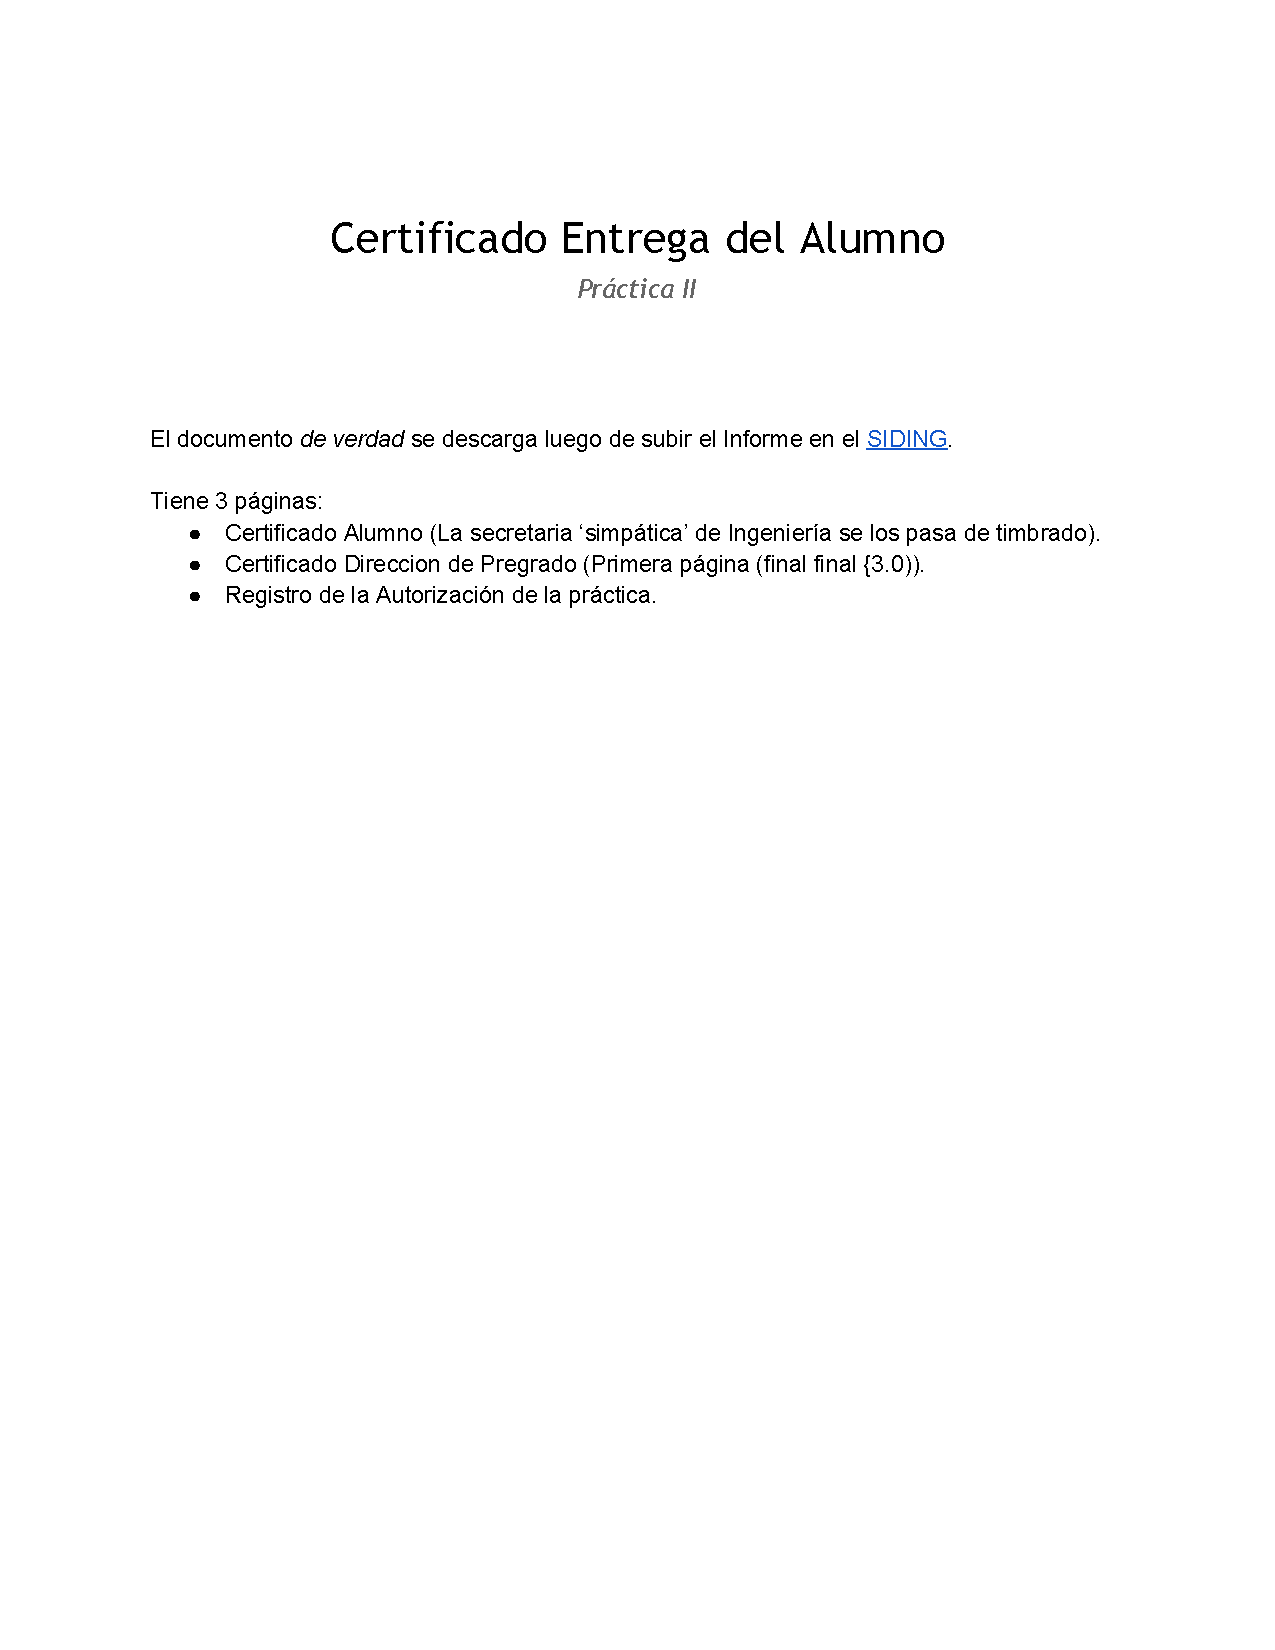
\includepdf[pages=-]{docs/cert.pdf}

\includepdf[pages=-]{docs/front.pdf}


% Evaluations
% -----------
% 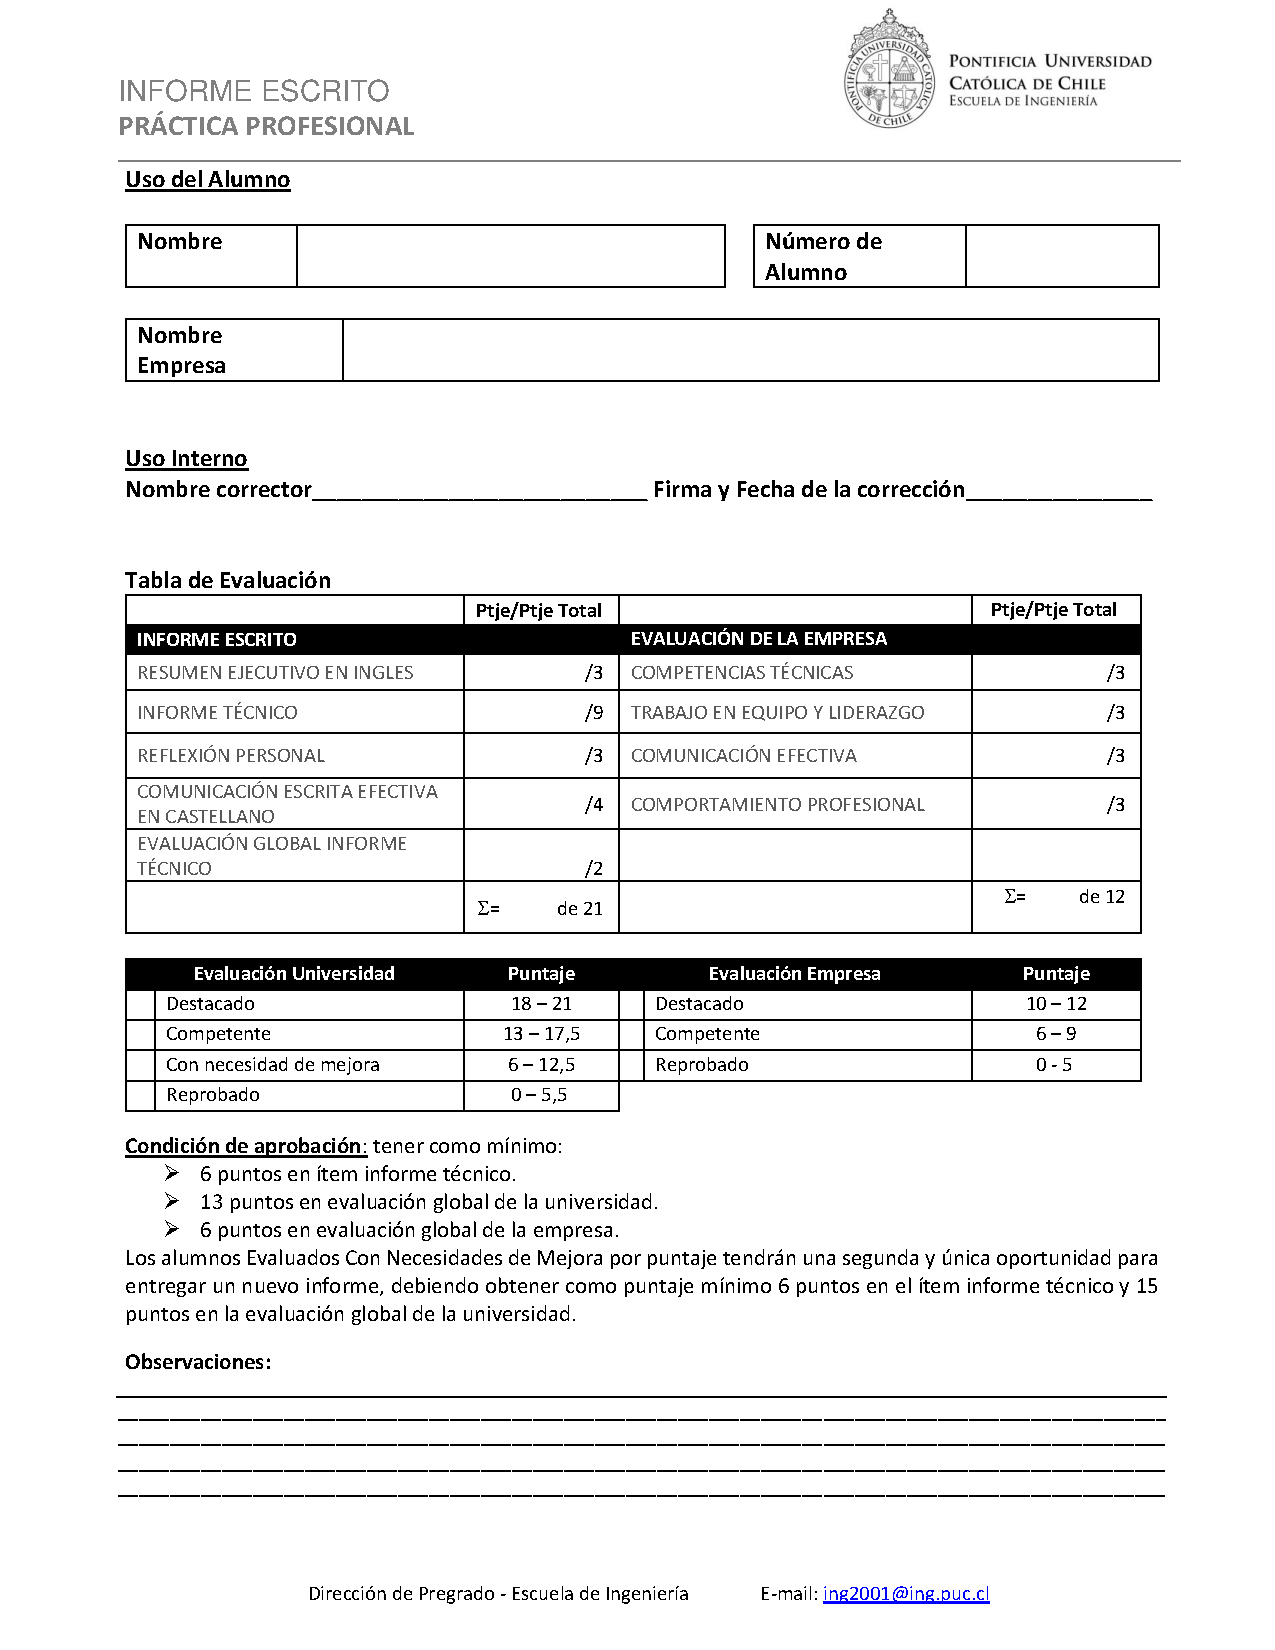
\includepdf[pages=-]{docs/university-evaluation.pdf}
% 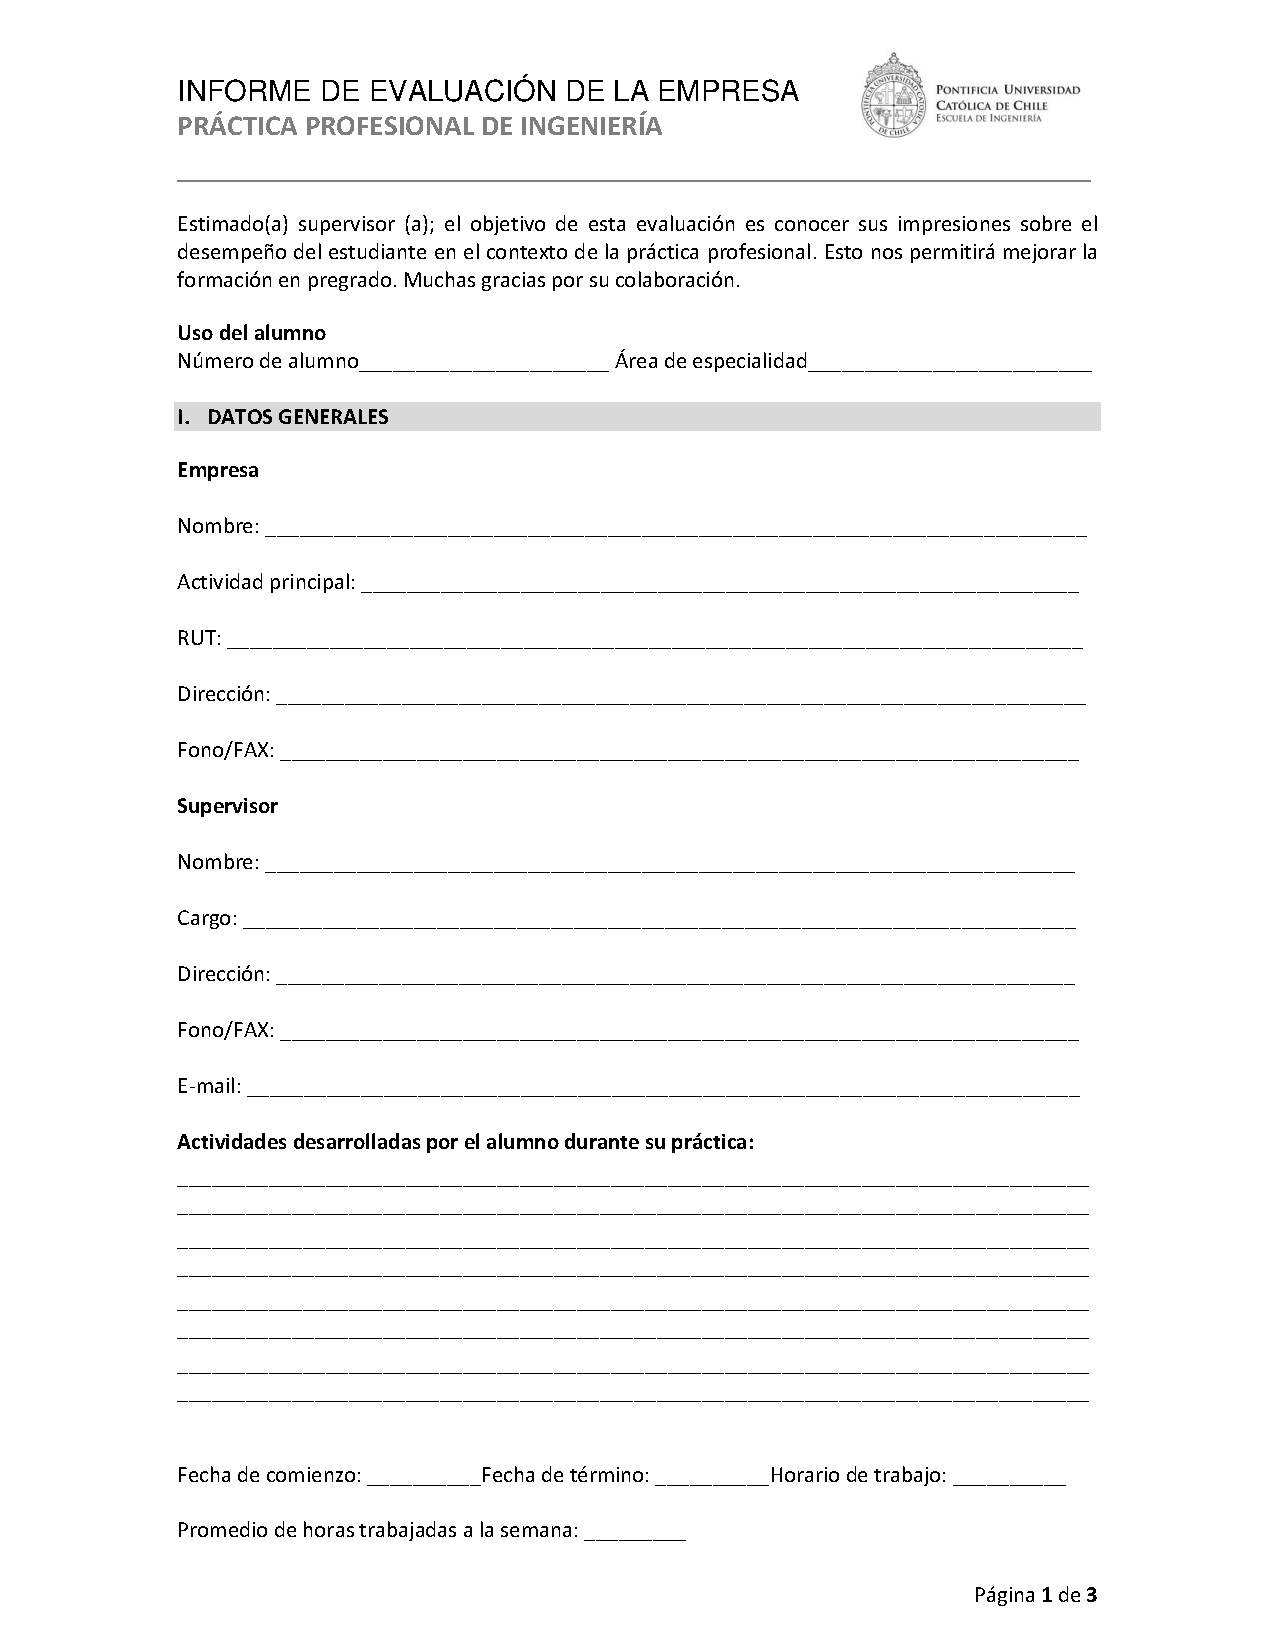
\includepdf[pages=-]{docs/internship-evaluation.pdf}


% Abstract
% --------
\pagenumbering{gobble}% Remove page numbers (and reset to 1)
% Resumen ejecutivo en inglés (Máximo una página)
% ===========================
%
% -Contextualiza el lugar de práctica (empresa, área) y el objetivo esperado al finalizar la práctica profesional.
% -Describe las principales actividades realizadas y las conclusiones del informe técnico.
% -Emplea un correcto uso de inglés cuidando la redacción y aspectos formales de la escritura (redacción (pls xd), ortografía y vocabulario).


\section*{Resumen ejecutivo}
\selectlanguage{British}  % Write like a sir.
This report details on the experience gathered from a whole summer wasted just to fill this document.
\selectlanguage{Spanish}
  % Abstract


% Indexes
% -------
\pagenumbering{arabic}% Arabic page numbers (and reset to 1)
% Content index stuff
% ===================
\newpage
\tableofcontents
\newpage
\listoftables
\newpage
\listoffigures


\section{Introducción}
\label{introduccion}
%!TEX root=main.tex
Rodrigo Moisés Stuardo Carvajal, persona natural y arquitecto de la Universidad de Chile, ``el cliente'', es dueño e inventor de la patente de invención con registro número 50.295 del Instituto Nacional de Propiedad Intelectual (INAPI), cuyo invento se denomina Sistema de Alcuza Integrada (SAI), que consiste en un nuevo sistema para organizar utensilios o envases dosificadores de especias líquidas y en grano que sirven para preparar, aliñar, condimentar y sazonar los alimentos. Se puede apreciar en la figura \ref{foto_alcuza} una imagen promocional de una alcuza fabricada a partir del SAI.

La génesis del SAI se encuentra en el año 2009 luego de identificar defectos en los sistemas tradicionales de alcuza y aceiteros, como por ejemplo el limitado control en las dosis servidas, goteo inevitable de su contenido, diseño sobrecargado, entre otros. Esto motiva la concepción del SAI y la consecuente construcción de prototipos para validar su recepción por parte del público, como los que se muestran en la figura \ref{foto_prototipos} del anexo \ref{anexo:figuras} \footnote{También existe un video explicativo publicado en \url{https://www.youtube.com/watch?v=uLd1JcDwyxE}}

El objetivo del Sr. Stuardo es enriquecer su imagen y carrera profesional de arquitecto, diseñador e inventor por medio del reconocimiento de sus pares diseñadores y de autoridades relacionadas, como también logrando tener éxito en la evolución de su invento en un producto de mercado. Este objetivo motivó su participación en el  “1$^{o}$  Concurso EnVase a Chile” el año 2009, donde destacó como finalista, y en la “4$^{o}$ Feria Innova” de Rancagua, donde también fue seleccionado en el área de diseño. Es aquí donde el Sr. Rodrigo decide proteger su creación, presentando la solicitud para patentarla en el INAPI como patente de Diseño Industrial, donde se determina posteriormente el valor de originalidad tanto en el país como en el mundo, que permitió clasificarla como Patente de Invención con vigencia de 20 años desde el 2009.

Para lograr la transferencia de su diseño al mercado el Sr. Rodrigo desea vender los derechos de propiedad intelectual a una persona o empresa que posea la capacidad de producir y también distribuir modelos de alcuza basados en el SAI a los consumidores; él no posee interés en su fabricación ni distribución. Destaca aquí, en el año 2009, la ocasión más cercana a consolidar la venta de la patente, cuando se llegó a un acuerdo con la empresa Bogaris S.A.
\footnote{
Bogaris S.A. es una empresa trasnacional con presencia en España, Portugal, Rumania y Bulgaria que centra sus actividades en parques comerciales, instalaciones y aceites de oliva ultravirgen, ver:
 \url{http://wwww.bogaris.com/es/bogaris/nuestra_empresa/index.html}

 }
 en que le comprarían la patente a 7 o 14 millones de pesos dependiendo del resultado obtenido en el “1er Concurso EnVase a Chile”. Si bien el SAI logró ser finalista del concurso, la empresa Bogaris S.A no volvió a comunicarse con el Sr. Rodrigo y la venta no se concretó. Desde entonces, el Sr. Rodrigo mantiene la hipótesis de que es necesario generar una primera línea de producción de alcuzas basada en el SAI para demostrar el valor de su invención a los inversionistas.

Si bien el Sr. Stuardo ha intentado participar en otros concursos de diseño al pie cuáles y vender su patente a otras empresas, ha enfrentado otras barreras que se lo han impedido. Algunas de éstas son: no tener un producto terminado, no ser una empresa con personalidad jurídica, y lo más importante, no tener una noción más precisa del precio al cual debiera venderse la patente ni argumentos que lo respalden. El objetivo de este trabajo es apoyar al Sr. Stuardo en su proceso de transformación del (diseño del) SAI en un producto de mercado mediante la aplicación de técnicas de evaluación de proyectos que permitan valorizar su patente y así determinar un precio de mercado para la patente. Esta valorización consiste en una primera etapa para alcanzar el objetivo del Sr. Stuardo, con la cual se espera apoyar su decisión de venta a un cliente específico mediante conclusiones basadas en datos consistentes y metodologías validadas de economía e ingeniería industrial.

En la sección \ref{diagnostico} se describe más detalladamente la invención y el estado actual del proyecto en el proceso de venta, como también aspectos relevantes sobre la regulación de propiedad industrial vigente en Chile y el mundo. Esto permite caracterizar un diagnóstico del proyecto basado en los análisis de FODA y fuerzas de Porter, y definir objetivos específicos para este estudio. Posteriormente, en la sección \ref{metodologia}, se discute una metodología de evaluación basada en los posibles mercados donde podría ingresar el SAI y la información pública disponible. Finalmente, en la sección \ref{analisis}, se analizan los resultados obtenidos, lo que permite concluir con recomendaciones finales en la sección \ref{conclusiones}. Adicionalmente, se incorpora un glosario de términos relevantes en el anexo \ref{glosario}, para facilitar el entendimiento del lector.


\section{Diagnóstico y objetivos}
\label{diagnostico}
%!TEX root=main.tex
\subsection{Descripción del SAI}

El SAI se define como un sistema de ensamble vertical de tres componentes, organizados para ajustarse entre sí y formar un Conjunto Contenedor, el SAI consta de dos Envases Individuales Dosificadores de productos líquidos o aceites comestibles los cuales incorporan un Atomizador para la dosificación de su contenido, estos envases son ensamblados por el tercer componente: Tapa Doble de Soporte interpuesta entre dichos envases individuales acoplados coaxial e invertidamente de forma vertical, que también funciona como un envase dosificador de especies en grano.

Este Conjunto Contenedor tiene la condición de Objeto de Invención (otorgada por la patente de INAPI N$^{o}$50.295, 22/10/2009) al desarmarse en componentes individuales como utensilios de cocina, y armarse en su forma integrada que permite que sus componentes se ajusten perfectamente formando un solo volumen que se puede manejar en forma inversa, para cambiar y elegir el envase que se desea utilizar.


\subsection{Sobre la propiedad intelectual}

La propiedad intelectual es una rama del derecho que fomenta la innovación, la creación y la transferencia tecnológica mediante la definición de derechos exclusivos sobre las invenciones o creaciones a cambio de que estas sean dispuestas al público general y que pasen a ser parte del dominio público luego de un tiempo determinado.  Un tipo particular de propiedad intelectual corresponde a la propiedad industrial, que corresponde a los derechos que una persona física o jurídica puede tener sobre una invención, las cuales se clasifican en: patentes de invención, modelos de utilidad, marcas comerciales, colectivas, de certificación e indicaciones geográficas y denominaciones de origen. El organismo encargado de administrar y atender los servicios asociados a la propiedad industrial es el INAPI. Además, existe el Tribunal de Propiedad Industrial (TDPI) como órgano jurisdiccional e independiente, el cual atiende las apelaciones sobre las resoluciones dictadas por el Director del INAPI.

A diferencia de otras formas de propiedad industrial, las invenciones se describen como “toda solución a un problema de la técnica que origine un quehacer industrial” (Ley 19039, art. 31) y deben caracterizarse por su novedad, nivel inventivo y aplicación industrial. En este caso, una patente de invención otorga protección sobre los derechos del propietario por un total de 20 años en el territorio del país, acerca del objeto de invención definido en la patente. Adicionalmente, el dueño de la patente permite registrar la propiedad industrial en los más de 200 países adheridos a la Organización Mundial de Propiedad Intelectual (OMPI) de forma más expedita, gracias al Tratado de Cooperación en materia de Patentes (PCT).

Respecto a la amplitud de la protección que otorga una patente de invención, la Ley 19039 especifica en el artículo 49 que ésta se determina por el contenido de la sección “reivindicaciones” de la patente misma, dejando la interpretación de la misma dependiendo de lo que se especifique en la sección “memoria descriptiva”. En el caso del SAI,  esto viene determinado por dos partes que se pueden resumir como: (1) todo conjunto coaxial compuesto de dos frascos idénticos mediante una tapa doble interpuesta entre éstos y (2) los detalles geométricos  expresados en las figuras que acompañan a la patente. La descripción más precisa del documento original se encuentra en el anexo \ref{memoria}
\footnote{Para profundizar en la interpretación de esta ley se ha coordinado una reunión con expertos en Propiedad Industrial del Centro de Innovación Anacleto Angelini.}.


Para realizar la venta de una patente, es decir, de los derechos de propiedad asociados a una patente de invención, normalmente se debe contactar al dueño para negociar la transferencia de estos ante el organismo correspondiente. No existe un organismo oficial encargado de gestionar el mercado de patentes, y aunque existen iniciativas privadas para realizar subastas , no existe información histórica disponible sobre el precio acordado y la fecha en que se consolidó.


Finalmente, es interesante notar que si bien la alcuza es un producto específico dentro de un surtido de productos de utensilios de cocina, como se ve en las figuras \ref{alcuzas_tiempo},
según la OMPI se han solicitado en promedio 4 patentes por año, destacando el año 2015, momento en que esta cifra se triplica.


\subsection{Diagnóstico y situación actual}

Se realizó un análisis de Fortalecas, Oportunidades, Debilidades y Amenazas para caracterizar el estado actual del proyecto, el cual se detalla en la figura \ref{foda1}. Se deduce a partir de éste que es necesario disminuir la incertidumbre en cuanto al valor de la patente. Al tener una buena estimación se eliminan en su mayoría las debilidades, puesto que no hay desconocimiento del precio posible, y amenazas, ya que se sabe si puede existir competencia de otros diseñadores o no.


\begin{figure}
  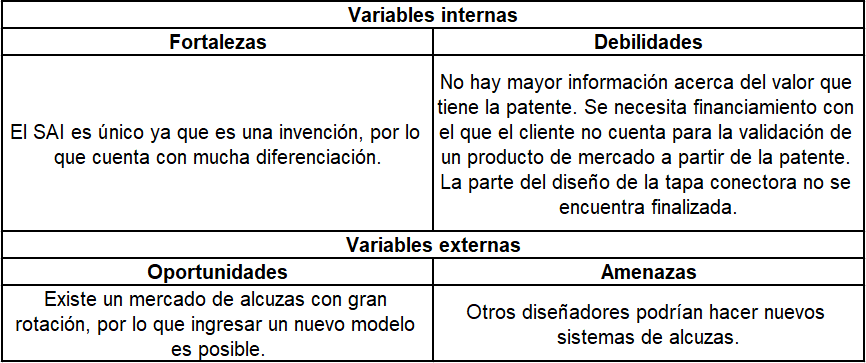
\includegraphics{FODA.png}
  \caption{Análisis FODA del proyecto de venta del SAI.}
  \label{foda1}
\end{figure}

Similarmente se realizó un análisis de las 5 fuerzas de Porter, el cual se detalla en la figura \ref{porter1}. Se ve a partir de esto, que el producto contiene un alto grado de diferenciación, pero existe una gran variedad de alcuzas tradicionales y no tradicionales disponibles en la competencia.

\begin{figure}
  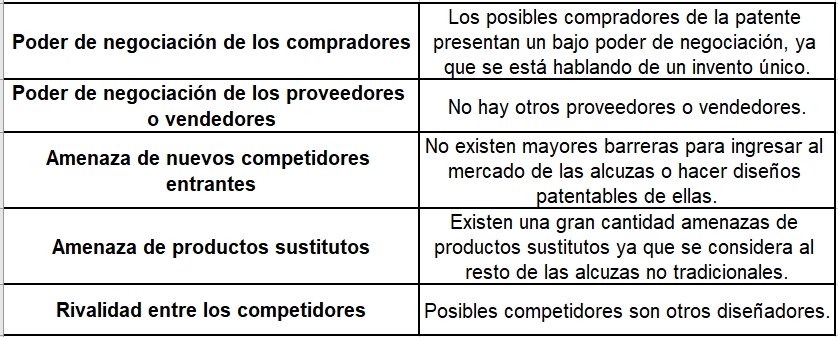
\includegraphics{Porter.png}
  \caption{Análisis de Porter del proyecto de venta del SAI.}
  \label{porter1}
\end{figure}

\subsection{Objetivos específicos de este trabajo}
\textbf{Objetivos Generales:}

Valorización de patente de invención de diseño de sistema de alcuza integrada INAPI registro N$^o$50.295 (22/10/2009)

Presentación de metodologías para la evaluación de patente de invención de diseño de sistema de alcuza integrada INAPI registro N$^o$50.295 (22/10/2009)



\textbf{Objetivos Específicos:}

Reducción de la incertidumbre en cuanto al precio de mercado que puede llegar a tener la patente INAPI  registro N$^o$50.295 (22/10/2009) para una posterior venta de los derechos de ella

Aumentar el marco de referencia que apoye la venta de patente de invención de diseño de sistema de alcuza integrada INAPI registro N$^o$50.295 (22/10/2009)


\section{Metodología}
\label{metodologia}
%!TEX root=main.tex
\subsection{Estrategia de valorización}
%!TEX root=main.tex
La valoración de una patente de invención presenta varios desafíos como se plantea en \url{http://users.ox.ac.uk/~mast0140/EJWP0599.pdf}. El primer de estos es que la comparación de su valor con el de otras patentes similares es muy riesgosa y suele no entregar resultados confiables. El segundo es que, naturalmente al ser un producto nuevo, existe muy poca información sobre cómo adoptarán el producto los consumidores y también el impacto que tendrá una determinada estrategia de marketing. Luego, como ni el método por comparación de mercado ni por múltiplos son válidos se debe valorizar mediante la estimación de los flujos actualizados para calcular el Valor Actualizado Neto (VAN) que le generará al dueño de la patente el poseer esta invención. Como al Sr. Stuardo sólo le interesa dedicarse a la producción de alcuzas basadas en el SAI, se decidió formular un negocio basado en una empresa que represente a un posible comprador que incorporará este diseño en su surtido de productos.

\subsection{Estimación de costos}
Se estima que se incurrirá en las siguientes inversiones y costos para la realización del proyecto:
\begin{itemize}
  \item Manufactura del producto: El costo estimado por unidad de alcuza es de 4000 pesos y este tiene un pedido mínimo de 50.000 unidades.

  \item Bodegaje del producto: Se considera el costo de oportunidad del uso de bodega. El precio de mercado por metro cuadrado es 0.14 UF (4254 pesos), con 4 metros de altura aproximadamente. El volumen del SAI es 0.002368 metros cúbicos y se considera un margen de seguridad del 10\% adicional para dar movilidad en el espacio.

  \item Despacho del producto: Se consideran costos de despacho (desde santiago) por unidad de volumen dependiendo de la región y de la demanda estimada, estos costos por región se obtuvieron de empresas de courrier nacionales

  \item Término del desarrollo de un producto en base al diseño de la patente: Para poder realizar la producción de alcuzas se necesita una matriz de producción, esta se puede elaborar mediante un Ingeniero civil mecánico y un matricero, sus costos son 2.000.000 y 1.000.000 de pesos respectivamente. Además es necesaria la elaboración de la matriz lo que tiene un costo de 1.500.000 de pesos.

  \item Costos fijos y gasto administrativos: se consideran costos anuales como un 10\% de la inversión inicial
\end{itemize}



\subsection{Estimación de ingresos}
%!TEX root=main.tex
\subsubsection{Definiciones previas}
En base al estudio de los distintos diseños de alcuza disponibles en el mercado se clasificaron los diseños en 2 tipos principales: tradicional y no tradicional. Los cuales se definen a continuación.

\textbf{Tradicional:} Se entiende por un diseño tradicional aquel que está compuesto por botellas de vidrio o cerámica, de color transparente o monocromático con tapa de madera,  vidrio o metal. En adición puede poseer una bombilla adaptada.

\textbf{No tradicional:} Un diseño no tradicional será todo aquel diseño que no se clasifica como tradicional. De acuerdo a aquello esta variante posee alguna característica innovadora respecto del modelo clásico dominante. Entre ellas se pueden mencionar una adaptación diferente para aplicar el contenido, diseño en la pintura o forma  creativa.

En  cuanto a la definición del cliente final de las alcuzas, la investigación que se muestra en siguiente inciso permitió determinar dos tipos:

\textbf{Clientes tipo 1:} personas que compran una alcuza para su casa o para regalo.

\textbf{Clientes tipo 2:} restaurantes que compran alcuzas para su negocio.

\subsubsection{Demanda: Levantamiento de información}

En la actualidad el registro de datos públicos acerca de la demanda de alcuzas es nulo. No existe información detallada sobre la participación de mercado de cada una, ni sobre el volumen que ofertan las empresas que venden este producto. Por dicha razón, se utilizaron distintas metodologías para estimar los datos faltantes, en específico se realizaron entrevistas y encuestas, las cuales se detallan a continuación.

\begin{itemize}
\item \textbf{Entrevistas a tiendas comerciales:}
\end{itemize}

Las entrevistas se realizaron con los siguientes objetivos: conocer la cantidad de alcuzas vendidas al mes; identificar proveedores; averiguar qué diseños que tienen a la venta y sus respectivos ciclos de vida en la tienda; e indagar sobre las principales características de las personas que compran alcuzas.

Hasta el momento se han entrevistado 6 tiendas distintas, Paris, Falabella, Ripley, Casa\&Ideas, Kitchen Republic y Capdor. Cabe mencionar que la totalidad de las tiendas estaban ubicadas en el Mall Costanera Center.

En el Anexo \ref{PauEntRetail} se detalla la pauta de preguntas que se utilizó. Dicha guía está sujeta a flexibilidades, dado que cada entrevista se orientó según variaciones surgidas en el momento.

Las respuestas obtenidas permiten concluir que el perfil general de clientes que compran alcuzas es variado. Se identificaron los siguientes motivos de compra: adquisición para luego regalarla, realizar una reposición o al momento de mudarse a una casa nueva. En cuanto a tasa de ventas, se determinó que la tienda Falabella vende alrededor de 15 alcuzas al mes durante noviembre y diciembre, y el resto del año vende aprox. 5 alcuzas al mes. Las tiendas Kitchen Republic y Casa\&ideas venden 40 y 20 unidades mensuales, respectivamente.  La tienda Capdor vende entre 15 y 20 alcuzas al mes. En adición, según estimaciones de la vendedora entrevistada de Falabella, la proporción de ventas de alcuzas tradicionales y no tradicionales es 8:2. En el Anexo \ref{ResEntRetail} se muestra la información de forma detallada.

Durante las visitas a tiendas comerciales se investigaron las marcas o fábricas y los países de fabricación de las alcuzas. En el Anexo \ref{MarAlc} se muestra la lista obtenida.

\begin{itemize}
\item \textbf{Entrevistas a restaurantes:}
\end{itemize}

Las entrevistas se realizaron con el objetivo de conocer la cantidad de alcuzas que poseen los restaurantes en relación a la cantidad de mesas, determinar cuántas veces al año realizan reposición de alcuzas, averiguar cuales son sus proveedores de alcuzas y de aceite, obtener una aproximación del dinero que están dispuestos a pagar por una alcuza y, por último, percibir opiniones acerca del diseño que se está evaluando y conocer disposición a pagar por este.

En el Anexo \ref{PauEntRest} se detalla la pauta seguida en estas entrevistas, hasta el momento se han entrevistado 12 restaurantes, 10 ubicados en Providencia y 2 en Isla de Maipo. Los locales entrevistados fueron: Barandiara, Parrillada del Chef, Voraz, Sandwicheria \& Bistro, Diddlers Irish Bar \& Restaurant, Le Fournil, Luca’s, My Tavuk, Shopdog, Normandie, El Rincón Rústico y Ziufande.


Las entrevistas permitieron concluir que aquellos restaurantes que forman parte de una cadena o franquicia no compran alcuzas, sino que sus proveedores se las regalan o venden a un mejor precio. Por otro lado, la porción de restaurantes que si compran alcuzas prefiere diseños tradicionales  frente al diseño de alcuza integrada. Entre las razones que mencionaron fue que poseen un diseño de alcuza fijo en el local y realiza compra para reponer su \textit{stock} de alcuzas, y un diseño no tradicional implica educar al cliente acerca de su uso.

En cuanto a datos cuantitativos, se determinó que cada restaurante posee aproximadamente 1 alcuza por mesa y que se realiza reposición de alcuzas una vez al año. En el Anexo \ref{ResResEntRest} se muestra una tabla resumen de los Resultados de las entrevistas. En forma adicional, en el Anexo \ref{ResEntRest} se muestran las respuestas de cada restaurante de forma detallada.

\begin{itemize}
\item \textbf{Encuestas a personas:}
\end{itemize}

Los principales objetivos de la encuesta son: obtener una estimación de la demanda de alcuzas en general; indagar si las personas conocen el producto y lo utiliza en su casa a diario; determinar el perfil de los posibles compradores del producto; conocer su comportamiento de compra y preferencias; y averiguar la disposición a comprar el diseño de alcuza integrada.

Las encuestas se realizaron en el camino entre la estación de metro Tobalaba y el centro comercial Mall Costanera Center, entre las 15:00 y 18:30 hrs. durante un día domingo. Cabe destacar que el sondeo abarcó a 57 personas.  En el  Anexo \ref{PauEnc} se detallan las preguntas realizadas. Para la posterior utilización de los datos se supuso que cada persona entrevistada representó a un hogar, debido a que el producto estudiado está presente en forma unitaria en las casas, esta última información se corroboró al momento de realizar la encuesta.

Las encuestas permitieron determinar que el 57,9\% de los encuestados poseen una alcuza en su casa. El 35,1\% de las personas encuestadas utiliza a diario la alcuza al momento de comer. En cuanto al comportamiento de compra se concluyó que el 33,4\% compró una alcuza hace menos de 3 años y el 26,4\% compró una alcuza durante el año 2016. En el Anexo \ref{ResEncPer}  se muestran las respuestas tabuladas.


\begin{itemize}
\item \textbf{Entrevistas a empresas de aceite:}
\end{itemize}

Los objetivos de las entrevistas a empresas productoras de aceite son: indagar acerca de sus proveedores de envases de vidrio, conocer la cantidad de envases de vidrio que compra la empresa mensualmente, determinar si la organización es proveedor directa de restaurantes, averiguar si la empresa cuenta con el servicio de venta o regalo de alcuzas a sus clientes y conocer la forma en que producen o compran las alcuzas.

Las organizaciones entrevistadas fueron Las Doscientas y Olivos Ruta del Sol, la primera fue realizada presencialmente mientras que la segunda se realizó mediante correo electrónico. En el Anexo \ref{PauEntEmpAce} se muestra la pauta de preguntas realizadas.

De las dos empresas entrevistadas, una empresa es proveedora directa de aceite de oliva a restaurantes, además posee su propio diseño de alcuza, el cual  vende a cierta cantidad de restaurantes en forma exclusiva. En adición se averiguó que el proveedor de envases de vidrio de ambas empresas es Cristalerías Toro. En el Anexo \ref{ResEntEmpAce} se muestran las respuestas detalladas de las entrevistas.

Cabe destacar que las entrevistas y encuestas sirvieron como una primera aproximación al mercado, y en el futuro se espera realizar más indagaciones de la misma forma que aporten mayor solidez a los datos obtenidos.

\subsubsection{ Participación de mercado}

Para determinar la participación de mercado se realizó el cálculo del porcentaje de ventas que corresponde a alcuzas tradicionales, para ello se utilizaron los datos obtenidos en las entrevistas a tiendas comerciales. Aquello permitió determinar qué aprox. el 80\% de las alcuzas vendidas corresponden a alcuzas de diseño tradicional y el resto no tradicional (esto para el caso de los locales que venden ambos tipos de diseño).

Se utilizó la venta mensual de alcuzas obtenida mediante de las entrevistas a tiendas comerciales, luego este dato se amplificó por la cantidad de sucursales que posee dicha tienda en la Región Metropolitana. Con ello se obtuvo una venta escalada a la región. Luego se determinó la cantidad total de ventas de alcuza tradicional con la suma ponderada de las ventas de la región con el 80\% correspondiente a porcentaje de alcuzas tradicionales a la venta. La cantidad total de ventas de alcuza no tradicional se calculó de forma similar, pero esta vez se ponderó la venta total por 20\%, correspondiente a las ventas de alcuzas no tradicionales. La Tabla \ref{PartMercAlcu} muestra los datos utilizados y resultados obtenidos.

\begin{table}[H]
\centering
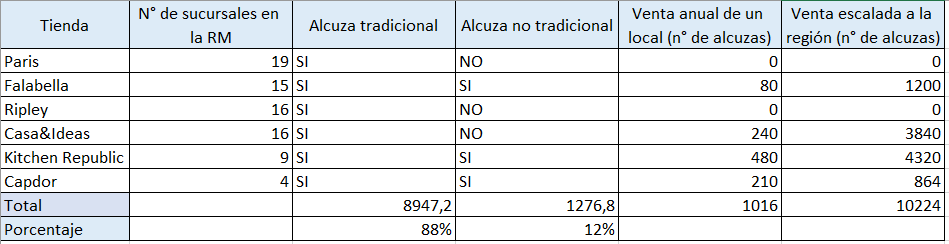
\includegraphics[width=\textwidth]{PartMercAlcu.png}
\caption{Participación de mercado de alcuzas, con datos obtenidos mediante entrevistas a tiendas.}
\label{PartMercAlcu}
\end{table}

Con los cálculos anteriores se determinó el porcentaje de ventas de alcuzas tradicionales el cual fue de 88\%, mientras que el porcentaje de venta de alcuzas no tradicionales es de 12\%.

Luego se utilizó la información disponibles de las páginas web de las principales tiendas  comerciales para determinar el promedio de alcuzas no tradicionales a la venta. Se estudió la gama de alcuzas que tienen a la venta las tiendas Falabella, Paris, Homy, Homecenter, Ripley, Casa\&Ideas, Easy, Morph, Kitchen Republic, Capdor, El Volcán, Imahe y Gangas. A partir de dicha información se determinó que el mercado, considerado en su totalidad, ofrece 48 diseños distintos de alcuzas tradicionales y 17 diseños de alcuzas no tradicionales. En el Anexo \ref{PartMerc} se encuentra la totalidad de datos tabulados.

Para estimar la participación del mercado que tendría la alcuza de sistema integrado se considera que esta debe ingresar al mercado y competir con las restantes alcuzas no tradicionales. Además, se supuso que no existe una preferencia significativa entre las distintas alcuzas no tradicionales, es decir, que la preferencia de los consumidores distribuye de forma uniforme entre los distintos tipos de diseños no tradicionales. Con todo lo anterior se concluye que la alcuza de sistema integrado utilizará 1/18  del mercado de alcuzas no tradicionales.

Por lo tanto el porcentaje que ocupará la alcuza integral dentro del mercado total del alcuzas será:

\begin{equation*}
\text{Porcentaje de participación de alcuza integrada} = 0.12 \times 100 \times \frac{1}{18} = 0.17\%
\end{equation*}

\subsubsection{Estimación de la demanda en la Región Metropolitana}

Las entrevistas realizadas a tiendas de retail permitieron determinar un periodo de 3 años para realizar el estudio. Además esto  se respalda por Estadísticas del Servicio de Impuestos Interno, las cuales afirman que la vida útil de enseres de vidrio de hoteles y restaurant tiene una duración de 3 años. \footnote{
Información disponible en \url{http://www.sii.cl/pagina/valores/bienes/tabla_vida_enero.htm} )
}
Para estimar la demanda, se consideraron por separado los dos tipos de cliente.
\paragraph{Demanda de Clientes tipo 1}

Para estudiar la demanda de clientes tipo 1 se propusieron dos metodologías, las cuales se detallan a continuación.

\textbf{Metodología 1:}  En base a información de encuestas a personas.

Para comenzar se realizará una estimación de la cantidad de hogares que existen en la RM.  Para ello se obtuvo un estimado de la población de la región y la cantidad de personas promedio por hogar, como se detalla a continuación.


Se obtuvo la población de los años 2017 a 2020 en las proyecciones del INE a partir del CENSO del año 2002  \cite{ine1}.

Se determinó el número de personas por hogar  según el CENSO del año 2002, el cual indica que en la Región Metropolitana este número es aproximadamente 3,75 \cite{ine2}. Se asumirá que este número es constante.

Con lo anterior se determinó la cantidad de hogares con la siguiente expresión:

\begin{equation*}
\mbox{N}^o\text{ de hogares} = \frac{\text{población en la Región Metropolitana}}{\text{Cantidad de personas por hogar}}
\end{equation*}

Luego, a partir, de la encuesta realizada se obtuvo la demanda anual con la pregunta n$^o$ 10 (ver Anexo \ref{PauEnc} y \ref{ResEncPer}). En ella se obtuvo el porcentaje de hogares que compró una alcuza durante el año 2016, con lo cual se obtuvo una estimación de la demanda anual de alcuzas. Dado que la cantidad de alcuzas que compraron durante el año 2016 fue de 16, equivalente al 28\% del total de personas encuestadas. En base a dichos datos se calculó la cantidad de hogares que compraría una alcuza en un año de la siguiente forma:


\begin{equation*}
\mbox{N}^o\mbox{ de hogares que compran} = \mbox{N}^o\mbox{ de hogares}\times 0,28
\end{equation*}

La expresión anterior representa la demanda total del alcuzas en un año.

Luego la cantidad de hogares que compran la alcuza integrada se determinará utilizando el porcentaje de participación del mercado determinada anteriormente (0,7\%). Los cálculos se muestran a continuación:

\begin{equation*}
\mbox{N}^o\mbox{ de hogares que compran alcuza integrada} = \mbox{N}^o\mbox{ de hogares que compran}\times 0,007
\end{equation*}

\textbf{Metodología 2:  Ciclo de vida del producto}

Dado el carácter de innovación del SAI se consideró que el Modelo de Bass era propicio para estudiar el ciclo de vida del producto.

La expresión matemática del modelo discreto es la siguiente:
\begin{equation*}
S_t=(P+Q(\frac{Y_{t-1}}{M}))(M-Y_{t-1}).
\end{equation*}
Donde $P_t$ es la citada probabilidad, $Y_{t-1} $ en número de compradores servidos hasta $t$ (o número de compradores acumulados en $t-1$) y $P$, $Q$ y $M$ son parámetros. Dado que $Y_0=0$, se cumple que $P_1=P$, es decir, $P$ es el parámetro que recoge el impacto inicial de la innovación, ya que determina la probabilidad de compra cuando todavía no existen usuarios previos; se denomina tasa de innovación. El parámetro $M$ expresa la población de potenciales usuarios del producto y se supone constante. Por lo tanto, $\frac{Y_{t-1}}{M}$ es la fracción de saturación del mercado en el período $t$. El parámetro $Q$ refleja el impacto de los usuarios previos sobre la probabilidad de compra y se denomina tasa de imitación o de difusión.


Referencias bibliográficas \cite{aleman2007estrategias} indican que el valor medio de $P$ está en torno a 0,02; mientras que el valor de $Q$ oscila entre 0,4 y 0,5. Por ello los parámetros utilizados para los cálculos fueron $P=0.02$ y $Q=0.45$ . El parámetro $M$ fue determinado como la cantidad de población que no posee una alcuza en su casa, esto se calculó con el porcentaje de personas que poseen alcuza en su casa (57.9\%, dato obtenido de la encuesta realizada), la predicción de la población de la región para los próximos 3 años y la probabilidad de comprar una alcuza (28\%,dato obtenido de la encuesta realizada). A continuación, se muestra la expresión para calcular el parámetro $M$.

\begin{equation*}
M=0,579\times 0,28 \times \mbox{Población de la región predicha para dicho año}
\end{equation*}

\paragraph{Demandas de clientes tipo 2}

Para el segundo tipo de clientes, los restaurantes, se puede comentar lo siguiente. Respecto a ellos las entrevistas señalaron que, en general, los restaurantes que cuentan con más de un local compran las alcuzas directamente a sus proveedores de aceites o estos últimos se los regalan por motivos de marketing. De la totalidad de restaurantes entrevistados que caen en esta categoría, sólo uno se mostró dispuesto a cambiar el producto tradicional por otro basado en el diseño que se está evaluando, sin embargo, señaló que solo lo compraría si el producto es más barato que el utilizado actualmente. Es por esta razón, que con los datos actuales que se tienen se concluyó que esta clase de restaurantes no adquirían este nuevo diseño de alcuza.

Los restaurantes más pequeños entrevistados compran las alcuzas al por mayor. Dos de ellos señalaron que podrían cambiar al diseño que se está evaluando, pero se mostraron reticentes a ello. Se cree que puede existir un tipo de restaurante que esté más interesado en este diseño, pero no se tienen datos de ello, por lo que solo se utiliza la demanda obtenida del primer tipo de cliente por el momento.

\subsubsection{Escalamiento de la demanda a Chile}

Para escalar los datos de la demanda hacia todo Chile se utilizó información acerca de la predicción de la población por cada región del país. Se obtuvo la población de los años 2017 a 2020 en las proyecciones del INE a partir del CENSO del año 2002.

Los cálculos para ambos casos fueron realizados de forma análoga a los mostrados en los incisos anteriores, a diferencia de que la predicción de la población de cada región fue propia de cada sitio.

En las tablas \ref{DemandaChileMet1} y \ref{DemandaChileMet2} se muestran los resultados obtenidos con las Metodologías 1 y 2 correspondientemente. En ellas se puede observar que mediante la Metodología 1 se estimó un total de 28.168 unidades de SAI demandadas, mientras que la Metodología 2 indicó un total de 49.718 unidades.

\begin{figure}[H]
\centering
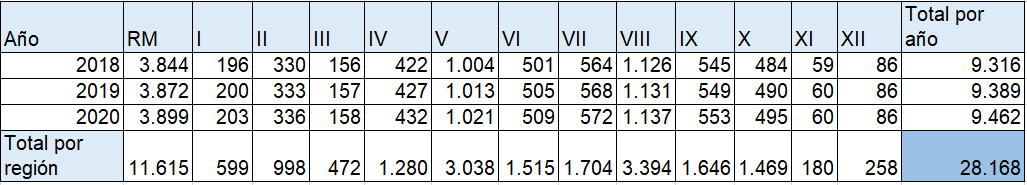
\includegraphics[width=\textwidth]{DemandaChileMet1.png}
\caption{Demanda en Chile, metodología 1.}
\label{DemandaChileMet1}
\end{figure}

\begin{figure}[H]
\centering
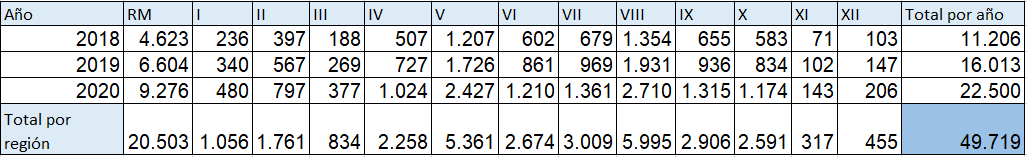
\includegraphics[width=\textwidth]{DemandaChileMet2.png}
\caption{Demanda en Chile, metodología 2.}
\label{DemandaChileMet2}
\end{figure}

\subsubsection{Precios de mercado}

Para determinar el precio de mercado de la alcuza integrada primero se obtiene el precio de venta de las alcuzas no tradicionales en las tiendas de retail. Luego, se estima el costo en adquirir dichas alcuzas a las tiendas. Dicho costo corresponde al precio al cual la empresa productora de alcuzas le vende el producto a las tiendas. A continuación se detalla el cálculo de cada paso.

En primer lugar se obtuvieron los precios de mercado de las alcuzas no tradicionales, esto se realizó a en base a catálogos de internet.  A partir de aquí se decide el precio al que se vendería la alcuza en el retail.

\begin{figure}[H]
\centering
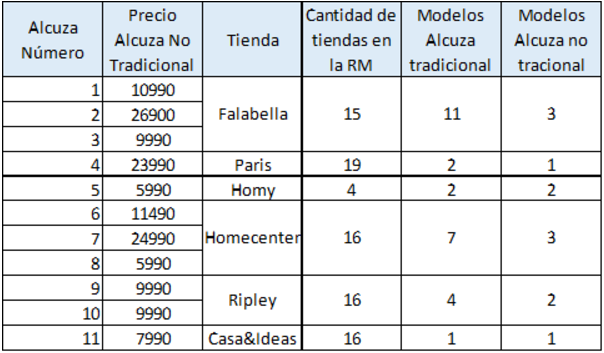
\includegraphics[scale=1.]{Precios.png}
\caption{Precios de las alcuzas no tradicionales.}
\label{Precios}
\end{figure}

Para determinar el precio al cual se venderá la alcuza, sin disponer de mayor información acerca del mercado y sus cuotas de distribución que los precios en las distintas tiendas, se plantea un problema básico de optimización de la cuota de mercado que se pretende alcanzar:
\begin{equation*}
\min \sum(P_i-P)^2
\end{equation*}

Donde $P_i$ es el precio de una alcuza no tradicional y $P$ es el precio al cual se venderá la alcuza integrada en el mercado. Tomando los datos de la Tabla \ref{Precios} el precio que maximiza la Cuota de Mercado Óptima (CMO) es \$14.175. La distribución de los precios y el óptimo se ve reflejada en la Figura \ref{GraficoPrecio}.

\begin{figure}[H]
\centering
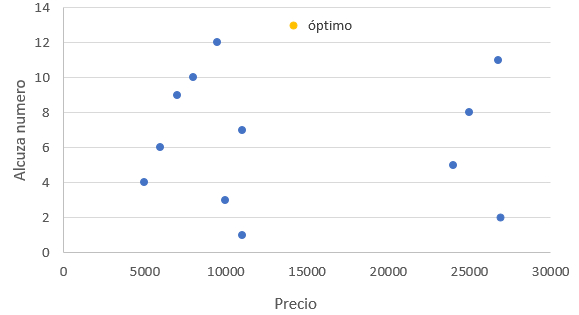
\includegraphics[scale=1.]{GraficoPrecio.png}
\caption{Determinación Cuota Mercado Óptima.}
\label{GraficoPrecio}
\end{figure}

Sin embargo, el modelo planteado debe implementar ciertas restricciones que se deben añadir al modelo una vez que se disponga de mayor información del mercado y además asume ciertos supuestos:
\begin{itemize}
\item Consumidores son racionales, demanda uniforme
\item Competencia no ajusta sus precios
\item Se debe considerar la elasticidad-precio de la demanda
\end{itemize}


En segundo lugar se determinó el porcentaje de costo sobre ingresos. Para este cálculo se utilizó el estado financiero de la tienda Fababella 2016 \cite{falabella}. En ella se muestra un de actividades ordinaria de 7.898.301.784 y un costo de ventas de 5.180.719.944, con lo que se obtiene que el costo de venta es el 66\% del ingreso por actividades ordinarias. Por lo tanto, el 66\% del precio óptimo de venta en retail es
\$$14.175 \times 0.66=\$9.355$, es decir, el precio de mercado de la alcuza integrada será de \$$9.355$.

Para obtener un costo más representativo se quiere seguir indagando en las empresas de retail, esto para obtener un margen promedio.

\subsubsection{Volumen a ofertar}

El volumen a ofertar del negocio que se está evaluando es el máximo entre el pedido mínimo que se puede mandar a hacer y la demanda estimada. Esto debido a que si no se hace el pedido mínimo se fabricarían 0 alcuzas, lo que sería equivalente a no producir, por lo que se tiene que producir al menos eso; y porque conviene producir a la demanda estimada si esta es mayor que el pedido mínimo.

Por un lado, se realizó una cotización a Cristalchile por el pedido mínimo que acepta, el cual es de 50.000. Por otro lado, la demanda total de alcuzas estimada mediante las 2 metodologías fue de 28.168 y 49.718 unidades, por lo que el volumen a ofertar será de 50.000 unidades.


\subsection{Tasa de descuento}
La tasa de descuento a utilizar es del 7,7\% considerando una industria de ventas comparable con el retail \cite{security}.


\section{Análisis de los resultados}
\label{analisis}
%!TEX root=main.tex
Según la metodología 1 el VAN del proyecto es $-\$16.580.118$, como el VAN es negativo podemos inferir que el proyecto no es rentable según la metodología 1, por otro lado el proyecto no tiene TIR ni período de payback.

Según la metodología 2 el VAN del proyecto es $\$33.833.974$, como el VAN es positivo podemos inferir que el proyecto es rentable según el modelo planteado. Su TIR y Payback son 20,27\% y 3 años respectivamente.

La diferencia entre las metodologías es la estimación de la demanda, siendo la segunda en la que se obtiene el mayor valor en ésta, lo que explica que se vendan más unidades y el VAN del proyecto sea positivo.

Esto revela la importancia que tiene lograr un buen posicionamiento del producto, debido a que hay una alta variación del valor del proyecto respecto a la demanda que se puede observar.

\subsection{Sensibilidad}

Se tomó la metodología 1 y se varió la cantidad de alcuzas no tradicionales con las que el producto derivado del SAI compartiría estante. Variar este parámetro se traduce en una variación de la participación de mercado, y es un indicador de qué tan demandado es el producto en comparación con otras alcuzas no tradicionales.

En la metodología 1, se estima que este parámetro es 17. El rango en que se varió en el análisis de sensibilidad fue entre 1 y 29, tomando solo valores discretos. Este rango se decició debido a que se desconoce qué tan demandado será el producto en comparación con su competencia más cercana de alcuzas no tradicionales. El detalle de los resultados se presenta en el Anexo \ref{AnSensibilidad1} y un gráfico resumen se presenta en la figura \ref{GraficoSensibilidad1}. Notemos que el VAN se hace 0 cuando este parámetro toma valores entre 13 y 14.

\subsection{Flexibilidad}

Un análisis de flexibilidad que se puede realizar es respecto a la empresa ficticia, dependiendo de si se ve obligada a comprar el lote completo de insumos para producir o si puede comprar la opción de comprar una fracción menor para así lanzar la primera producción, probar la recepción en el mercado, y luego decidir si pedir la otra fracción del lote. Llamamos a esta opción la de flexibilidad número 1. Esto se representa en la figura \ref{flexibilidad}, donde $q$ es la probabilidad de tener éxito con el primer volumen de producción y $r$ la probabilidad de tener éxito en el segundo, asumiendo que se decidió producir el primero.

\subsection{Sustentación}

La sustentación del proyecto está en que se trata de una invención, por lo que el producto final puede variar en esta idea y sus distintas versiones pueden perdurar en el mercado de forma que su ciclo de vida es mayor a la de un producto único. Por otro lado, como se consideró una empresa ficticia, ésta ya posee una estabilidad económica y una solidez, que permite aquellos periodos en que la demanda no se comportó como lo esperado y se pueda mantener el proyecto.


\section{Conclusiones}
\label{conclusiones}
%!TEX root=main.tex
Se ha definido un modelo para la valorización de la patente de invención que indica los parámetros más relevantes a tener en consideración al momento de evaluar o ejecutar el proyecto.

La diferencia entre las metodologías en la estimación de los perfiles de demanda, permite identificar que el éxito del proyecto depende en gran medida del valor real y es en donde se debe hacer el mayor esfuerzo de estimación. Un análisis de mercado más detallado encargado a algún agente externo permitiría conocer con mayor precisión el valor esperado de la demanda, por lo que sería relevante conocer a priori el costo de realizar dicho estudio.

También es relevante en esta evaluación la cantidad inicial de unidades producidas ya que en ambos escenarios, la demanda total es menor a esta cantidad, actualmente se considera la restricción de pedido minimo del proveedor local, actualmente se espera la respuesta por parte de proveedores de China que tienen mayor holgura en dicha cantidad, pero con la consiguiente diferencia en la estructura de costos al considerarse por ejemplo costos de envío.


Por otro lado el presente trabajo se limita a la evaluación económica del proyecto considerando las variables más relevantes asociadas a este, sin embargo se deben considerar las distintas líneas de financiamiento para el cliente en particular ya que de conseguirse le permitirían completar el desarrollo del producto además de generar un MVP y con ello tener un parámetro más acotado para los costos y poder presentar el proyecto ante posibles compradores, inversionistas, patrocinadores o asociaciones con marcas.

Se recomienda la presentación de los resultados de esta evaluación a entidades que podrían estar interesadas en la compra de los de derechos de la patente. En conjunto con esto se recomienda al cliente finalizar el diseño de la tapa conectora para poder tener un diseño completo que presentar.


% References
% ----------
\renewcommand\bibsection{\section{\refname}}
\bibliographystyle{alpha}
\bibliography{references}


% Appendix
% --------
\newpage

\appendix
\section{Anexos}

\subsection{Glosario de conceptos relevantes }
\label{glosario}
\begin{itemize}
\item Alcuza:   (del árabe hispánico «alkúza», a su vez del árabe clásico «kūzah», y este del arameo «kūz[ā]», y este del persa «kuze») es una vasija para almacenar y administrar el aceite. El término alcuza se ha perdido en favor del más general aceitera, que puede denominar aceiteras, vinagreras y juegos de recipientes para aliñar las ensaladas.Pieza con dos frascos para aceite y vinagre).
\item Atomizar:         	Dividir algo en partes sumamente pequeñas, pulverizar.
\item Concepto:        	Idea que concibe o forma el entendimiento.
Conjunto contenedor	Un agregado de varias cosas que llevan o encierran dentro de sí a otras.
Diseño  Concepción original de un objeto u obra destinados a la producción en serie.
\item Diseño industrial:          	Proceso de diseño aplicado a los productos que se van a fabricar mediante técnicas de producción en masa.
Dispensador (distribuir) Dividir o repartir una cosa, señalando lo que corresponde a cada parte.
\item Dosificar:          	Dividir o graduar la cantidad o porción de algunas cosas.
\item Ensamble:        	Conjunto de piezas unidas, juntadas y/o ajustadas entre sí.
Envase. Recipiente o vaso en que se conservan y transportan ciertos géneros. Aquello que envuelve o contiene artículos de comercio u otros efectos para conservarlos o transportarlos.
\item Ergonomía:      	Estudio de la adaptación de las máquinas, muebles y utensilios a la persona que los emplea habitualmente, para lograr una mayor comodidad y eficacia.
\item Idea:   	Primero y más obvio de los actos del entendimiento, que se limita al simple conocimiento de algo. Imagen o representación que del objeto percibido queda en la mente.
\item Innovación:     	Es la creación o modificación de un producto o proceso y su introducción en un mercado que a su vez soluciona un problema de la técnica.
\item Integrado:       	Dicho de un conjunto de objetos: que constituyen un todo.
\item Invención:       	Es una solución nueva a un problema técnico, que genera actividad industrial, pudiendo dicha solución estar dada por un producto o un procedimiento. Para obtener una patente de invención, la invención debe ser nueva, inventiva y susceptible de aplicación industrial.
\item Maqueta:         	 Montaje funcional, a menor o mayor escala de un objeto, artefacto u edificio, realizada con materiales pensados para mostrar su funcionalidad, volumetría, mecanismos internos o externos o bien para destacar aquello que, en su escala real, una vez construido o fabricado, presentará como innovación o mejora.
Materialidad  	Superficie exterior o apariencia de las cosas. Se refiere al material básico de composición del objeto.
\item Packaging:       	Un recipiente o envoltura que contiene productos de manera temporal principalmente para agrupar unidades de un producto pensando en su manipulación, transporte y almacenaje.
\item Patente: Es un derecho de exclusividad, concedido por el Estado, para proteger y explotar una invención por el tiempo que determine la Ley.
\item PET:    	es un tipo de plástico muy usado en envases de bebidas y textiles.
\item Plástico: Dicho de ciertos materiales sintéticos: Que pueden moldearse fácilmente  y están compuestos principalmente por polímeros, como la celulosa.
\item Producción en Serie:    	Proceso en la producción industrial cuya base es la cadena de montaje o línea de ensamblado o línea de producción; una forma de organización de la producción que delega a cada trabajador una función específica y especializada en máquinas también más desarrolladas.
\item Producto de mercado:    Una opción elegible, viable y repetible que la oferta pone a disposición de la demanda, para satisfacer una necesidad o atender un deseo a través de su uso o consumo.
\item Prototipo:        	Un ejemplar o primer molde en que se fabrica una figura u otra cosa.
\item Pulverizar:       	Esparcir un líquido en partículas muy tenues, a manera de polvo
\item PVC:    	es el producto de la polimerización del monómero de cloruro de vinilo.
\item Recipiente.:    	Utensilio destinado a guardar o conservar algo.
\item Sistema industrial:        	Sistema que proporciona una estructura que agiliza la descripción, la ejecución y el planteamiento de un proceso industrial
Sistema Conjunto de cosas que relacionadas entre sí ordenadamente contribuyen a determinado objeto.
Tapa  	Pieza que cierra por la parte superior cajas o recipientes.
\item Utensilio de cocina:      	Es una herramienta que se utiliza en el ámbito culinario para la preparación de los platos.
\item Válvula: Mecanismo que regula el flujo de la comunicación entre dos partes de una máquina o sistema. Mecanismo que impide el retroceso de un fluido que circula por un conducto.
\item Vidrio:	Material duro, frágil y transparente o translúcido, sin estructura  cristalina, obtenido por la fusión de arena silícea con potasa y moldeable a altas temperaturas.
\end{itemize}


\newpage
\subsection{Tablas}
\begin{table}[hb]
\centering
\begin{tabular}{|l|l|}
\hline
\rowcolor[HTML]{DDEBF7}
Nombre de la subasta  & Sitio web                                                                    \\ \hline
IP Offerings          & \url{http://www.ipofferings.com/patent-value-quotient.html}                \\ \hline
Patent Auction        & \url{https://www.patentauction.com/}                                       \\ \hline
e-bay patents         & \url{https://www.ebay.com/b/Patents-Trademarks-for-Sale} \\ \hline
Ocean Tomo            & \url{http://www.oceantomo.com/auctions/}                                   \\ \hline
ICAP Patent Brokerage & \url{http://icappatentbrokerage.com/}                                      \\ \hline
\end{tabular}
\caption{Ejemplos de sitios web de empresas que gestionan subastas de patentes.}
\label{sitios_de_subastas}
\end{table}
\newpage
\subsection{Figuras}
\label{anexo:figuras}
% \begin{figure}[hb]
%   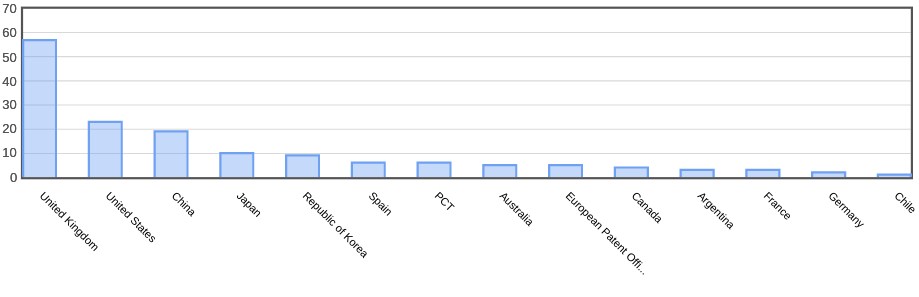
\includegraphics[width=\textwidth]{cruet_patents_country.png}
%   \label{alcuzas_paises}
%   \caption{Número de patentes solicitadas por país desde enero de 2007 a la fecha por país y que contienen \textit{alcuza} o \textit{cruet} en su portada, según la base de datos de la Organización Mundial de Propiedad Intelectual.}
% \end{figure}
\begin{figure}[hb]
  \centering
  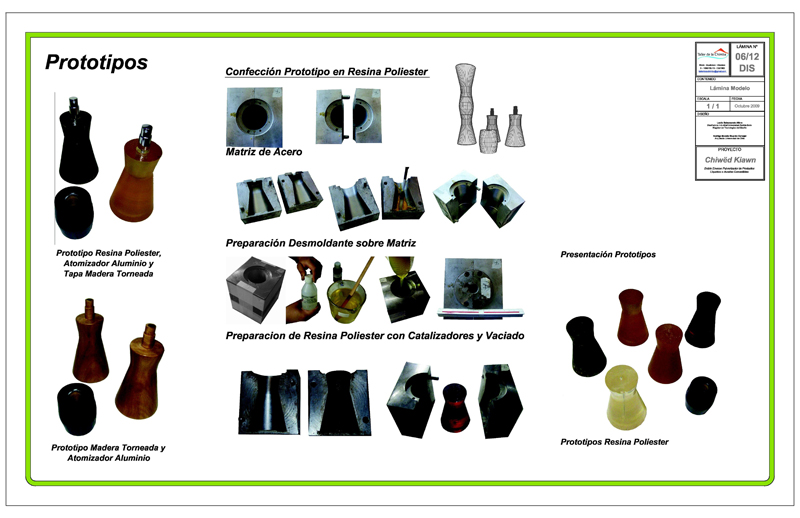
\includegraphics[width=\textwidth]{prototipos.jpg}
  \caption{Prototipos elaborados del diseño de Sistema de Alcuza Integrada (SAI) y algunas herramientas utilizadas.}
  \label{foto_prototipos}
\end{figure}

\begin{figure}
  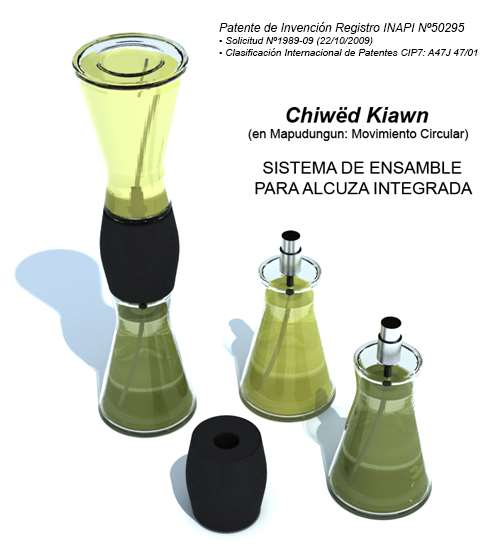
\includegraphics{alcuza.png}
  \caption{Imagen promocional (foto-montaje) de una alcuza fabricada a partir del SAI.}
  \label{foto_alcuza}
\end{figure}
\begin{figure}[hb]
  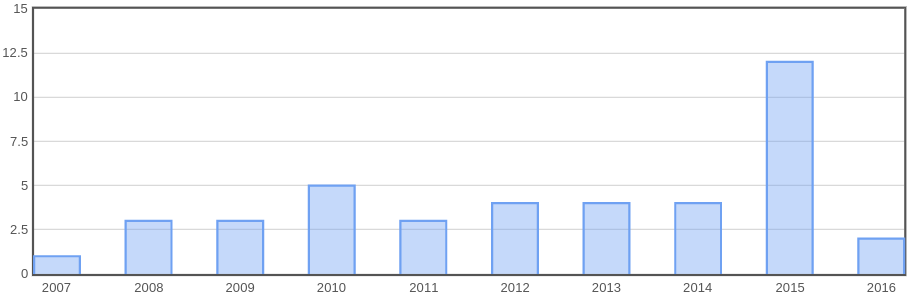
\includegraphics[width=\textwidth]{cruet_patents_time.png}
  \caption{Evolución del número de patentes solicitadas desde enero de 2007 a la fechas que contienen \textit{alcuza} o \textit{cruet} en su portada, según la base de datos de la Organización Mundial de Propiedad Intelectual.}
  \label{alcuzas_tiempo}
\end{figure}
\begin{itemize}
\item Alcuza:   (del árabe hispánico «alkúza», a su vez del árabe clásico «kūzah», y este del arameo «kūz[ā]», y este del persa «kuze») es una vasija para almacenar y administrar el aceite. El término alcuza se ha perdido en favor del más general aceitera, que puede denominar aceiteras, vinagreras y juegos de recipientes para aliñar las ensaladas.Pieza con dos frascos para aceite y vinagre).
\item Atomizar:         	Dividir algo en partes sumamente pequeñas, pulverizar.
\item Concepto:        	Idea que concibe o forma el entendimiento.
Conjunto contenedor	Un agregado de varias cosas que llevan o encierran dentro de sí a otras.
Diseño  Concepción original de un objeto u obra destinados a la producción en serie.
\item Diseño industrial:          	Proceso de diseño aplicado a los productos que se van a fabricar mediante técnicas de producción en masa.
Dispensador (distribuir) Dividir o repartir una cosa, señalando lo que corresponde a cada parte.
\item Dosificar:          	Dividir o graduar la cantidad o porción de algunas cosas.
\item Ensamble:        	Conjunto de piezas unidas, juntadas y/o ajustadas entre sí.
Envase. Recipiente o vaso en que se conservan y transportan ciertos géneros. Aquello que envuelve o contiene artículos de comercio u otros efectos para conservarlos o transportarlos.
\item Ergonomía:      	Estudio de la adaptación de las máquinas, muebles y utensilios a la persona que los emplea habitualmente, para lograr una mayor comodidad y eficacia.
\item Idea:   	Primero y más obvio de los actos del entendimiento, que se limita al simple conocimiento de algo. Imagen o representación que del objeto percibido queda en la mente.
\item Innovación:     	Es la creación o modificación de un producto o proceso y su introducción en un mercado que a su vez soluciona un problema de la técnica.
\item Integrado:       	Dicho de un conjunto de objetos: que constituyen un todo.
\item Invención:       	Es una solución nueva a un problema técnico, que genera actividad industrial, pudiendo dicha solución estar dada por un producto o un procedimiento. Para obtener una patente de invención, la invención debe ser nueva, inventiva y susceptible de aplicación industrial.
\item Maqueta:         	 Montaje funcional, a menor o mayor escala de un objeto, artefacto u edificio, realizada con materiales pensados para mostrar su funcionalidad, volumetría, mecanismos internos o externos o bien para destacar aquello que, en su escala real, una vez construido o fabricado, presentará como innovación o mejora.
Materialidad  	Superficie exterior o apariencia de las cosas. Se refiere al material básico de composición del objeto.
\item Packaging:       	Un recipiente o envoltura que contiene productos de manera temporal principalmente para agrupar unidades de un producto pensando en su manipulación, transporte y almacenaje.
\item Patente: Es un derecho de exclusividad, concedido por el Estado, para proteger y explotar una invención por el tiempo que determine la Ley.
\item PET:    	es un tipo de plástico muy usado en envases de bebidas y textiles.
\item Plástico: Dicho de ciertos materiales sintéticos: Que pueden moldearse fácilmente  y están compuestos principalmente por polímeros, como la celulosa.
\item Producción en Serie:    	Proceso en la producción industrial cuya base es la cadena de montaje o línea de ensamblado o línea de producción; una forma de organización de la producción que delega a cada trabajador una función específica y especializada en máquinas también más desarrolladas.
\item Producto de mercado:    Una opción elegible, viable y repetible que la oferta pone a disposición de la demanda, para satisfacer una necesidad o atender un deseo a través de su uso o consumo.
\item Prototipo:        	Un ejemplar o primer molde en que se fabrica una figura u otra cosa.
\item Pulverizar:       	Esparcir un líquido en partículas muy tenues, a manera de polvo
\item PVC:    	es el producto de la polimerización del monómero de cloruro de vinilo.
\item Recipiente.:    	Utensilio destinado a guardar o conservar algo.
\item Sistema industrial:        	Sistema que proporciona una estructura que agiliza la descripción, la ejecución y el planteamiento de un proceso industrial
Sistema Conjunto de cosas que relacionadas entre sí ordenadamente contribuyen a determinado objeto.
Tapa  	Pieza que cierra por la parte superior cajas o recipientes.
\item Utensilio de cocina:      	Es una herramienta que se utiliza en el ámbito culinario para la preparación de los platos.
\item Válvula: Mecanismo que regula el flujo de la comunicación entre dos partes de una máquina o sistema. Mecanismo que impide el retroceso de un fluido que circula por un conducto.
\item Vidrio:	Material duro, frágil y transparente o translúcido, sin estructura  cristalina, obtenido por la fusión de arena silícea con potasa y moldeable a altas temperaturas.
\end{itemize}

\newpage

\subsection{Memoria descriptiva de la patente del SAI}
\label{memoria}
\vspace{7cm}
\begin{center}

  Este espacio fue dejado en blanco intencionalmente.
\end{center}

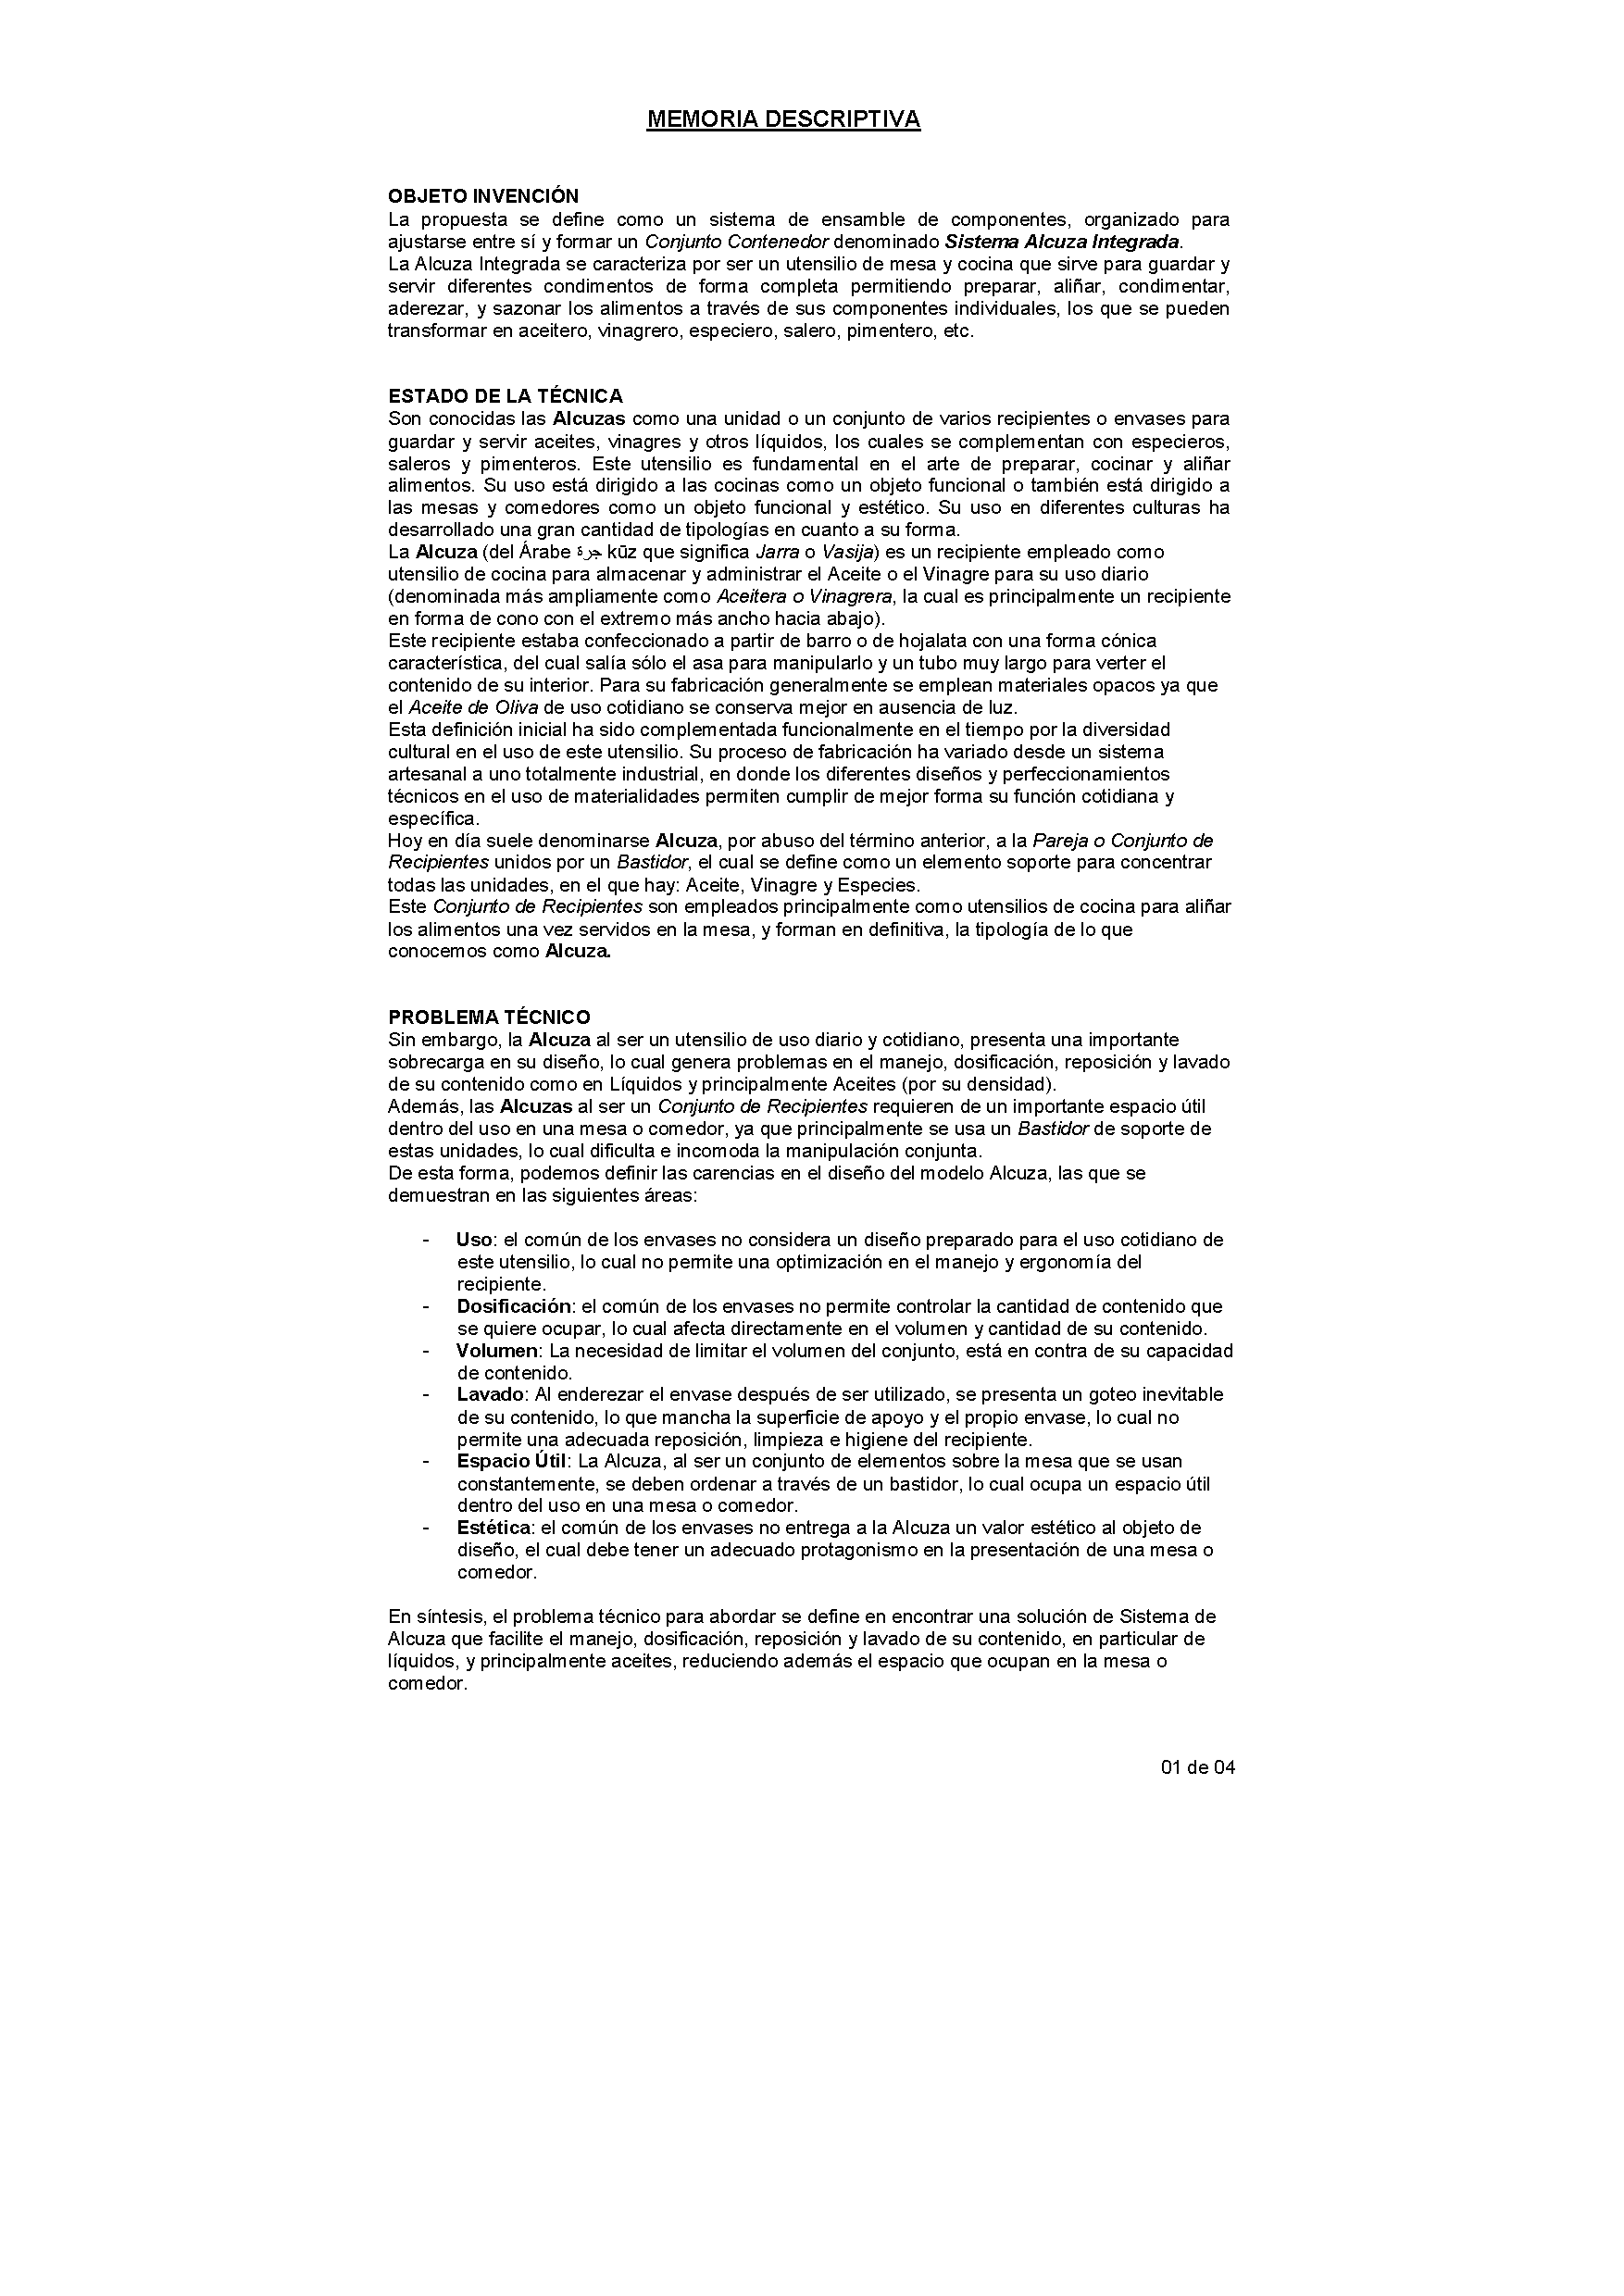
\includepdf[pages=-,frame,scale=0.9]{graphics/memoria_patente.pdf}

\newpage
\subsection{ Pauta de preguntas para entrevistas a tiendas comerciales.}
\label{PauEntRetail}

\begin{enumerate}
\item Aproximadamente ¿cuántas alcuzas vende al mes?
\item ¿Cuantos diseños diferentes tiene a la venta su tienda actualmente?
\item ¿Cada cuanto tiempo se cambia el mix de alcuzas que se vende en la tienda?
\item ¿Podría definir un perfil específico para las personas que compran alcuzas?
\end{enumerate}

\newpage
\subsection{Resultados de entrevistas a tiendas comerciales.}
\label{ResEntRetail}

\textbf{Paris.}

\begin{itemize}
\item Cantidad de diseños diferentes de alcuzas a la venta: 1.
\item El encargado de ventas indica que la venta de alcuzas es “casi nula” y recomendó buscar en tiendas especializadas o Falabella tal vez.
\end{itemize}

\textbf{Falabella.}

La vendedora indica distintas afirmaciones según su experiencia adquirida en el tipo que lleva trabajando en la tienda:
\begin{itemize}
\item Afirma que los clientes “compran harto para armar una casa o cuando están remodelando cocina por ejemplo”.
\item El perfil de clientes son “varones separados”, “parejas jóvenes argentinas”.
\item Para el caso de los hombres, estos buscan calidad más que precio. Al contrario, las mujeres priorizan el precio.
\item La vendedora lleva 4 meses trabajando y no han cambiado ninguna alcuza de las repisas.
\item En cuanto a las ventas afirma que “por mes venden aprox.15 (noviembre y diciembre), el resto del año a lo más 5 por mes”.
\item Afirma que “las alcuzas se venden más en época de navidad, como regalo. El resto del año es muy poco lo que se vende. Este año para navidad tuvieron un diseño de \$26.000 que se vendió harto,había una de \$15.000 también, el resto no se vendió”.
\item Principales marcas de alcuzas: Basement - Propaga.
\item La proporción de venta entre alcuzas tradicionales y no tradicionales es alrededor de 8:2.
\end{itemize}

\textbf{Ripley.}

\begin{itemize}
\item Cantidad de diseños diferentes de alcuzas a la venta: 1.
 \item La vendedora afirma que desde marzo que no ha vendido ninguna alcuza.
\end{itemize}

\textbf{Casa\&ideas.}

El vendedor responde según su experiencia en el tiempo que lleva trabajando en la tienda:

\begin{itemize}
\item Se vende más la alcuza compuesta por varios recipientes que la alcuza de una sola botella.
\item Aproximadamente de venden 20 unidades de alcuzas al mes.
\item ”El perfil de clientes que compran alcuzas es muy variado”.
\item Lleva dos meses trabajando en la tienda y ha visto el mismo modelo de alcuza durante todo ese tiempo.
\end{itemize}

\textbf{Kitchen republic.}

La vendedora responde según la experiencia adquirida durante el tiempo que lleva trabajando en la tienda.

\begin{itemize}
\item Venden aproximadamente 40 alcuzas al mes.
\item ”Lo compra todo tipo de gente”.
\end{itemize}

\textbf{Capdor.}

El vendedor responde según la experiencia adquirida durante el tiempo que lleva trabajando en la tienda.

\begin{itemize}
\item Cantidad de diseños diferentes de alcuzas a la venta: entre 6 y 8.
\item Se cambian los diseños de alcuzas a la venta 2 o 3 veces al año.
\item Al mes se venden entre 15 y 20 alcuzas.
\item El principal motivo de compra es por regalo o reposición.
\item La alcuza más vendida es un producto chileno, de Cristal Art.
\end{itemize}


\newpage
\subsection{Marcas y países de fabricación de alcuzas}
\label{MarAlc}
\begin{table}[H]
\centering
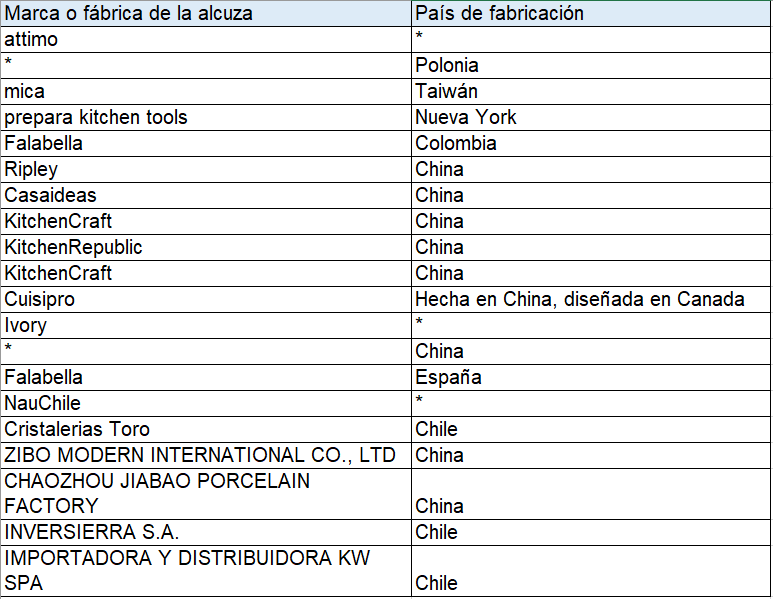
\includegraphics[scale=1.]{Marcas.png}
\caption{Marcas y países de fabricación de alcuzas.Simbología: *;no hay información disponible.}
\label{Marcas}
\end{table}

\newpage

\subsection{Entrevista a restaurantes - Pauta de preguntas}
\label{PauEntRest}

\begin{enumerate}
\item ¿Posee alcuzas en su restaurante?
\item ¿Cuántas mesas posee en su local?
\item ¿Cuántas alcuzas posee en su local?
\item ¿Durante el año 2016 cuántas veces realizó un reposicion de alcuzas?
\item ¿Con qué frecuencia realiza una reposición de alcuzas?
\item. La última vez que compró alcuzas, ¿a qué tienda fue? ¿Cuántas compró? ¿Algo que recalcar de la compra? (A qué tienda fue, cuantas compro aprox, etc, dejar que se explaye lo más posible, para entender cómo funciona la compra)
\item ¿Posee algún proveedor específico?
\item ¿Cuánto dinero gastó en su última compra de alcuzas? (monto por alcuza si es posible o monto total)
\item ¿Qué monto considera apropiado para pagar por una alcuza?
\item Al momento de realizar la compra, ¿en qué características se enfocó para hacer su elección?
\item ¿Estaría dispuesto a cambiar su set de alcuzas habituales por este nuevo modelo? (explicar diseño) (referenciar imagen)
\item ¿Cuál cree usted que es el valor de este nuevo modelo?
\begin{itemize}
\item[a)] Desde \$0 hasta  \$4.000
\item[b)] Más de \$4.000 hasta  \$8.000
\item[c)] Más de \$8.000 hasta \$12.000
\item[d)] Más de \$12.000 hasta \$16.000
\item[e)] Más de \$16.000 hasta \$20.000
\item[f)] Más de \$20.000
\end{itemize}
\end{enumerate}

\newpage
\subsection{Resumen de resultados de entrevistas a restaurantes.}
\label{ResResEntRest}

\begin{table}[H]
\label{ResumenEntrevistasRestaurantes}
\centering
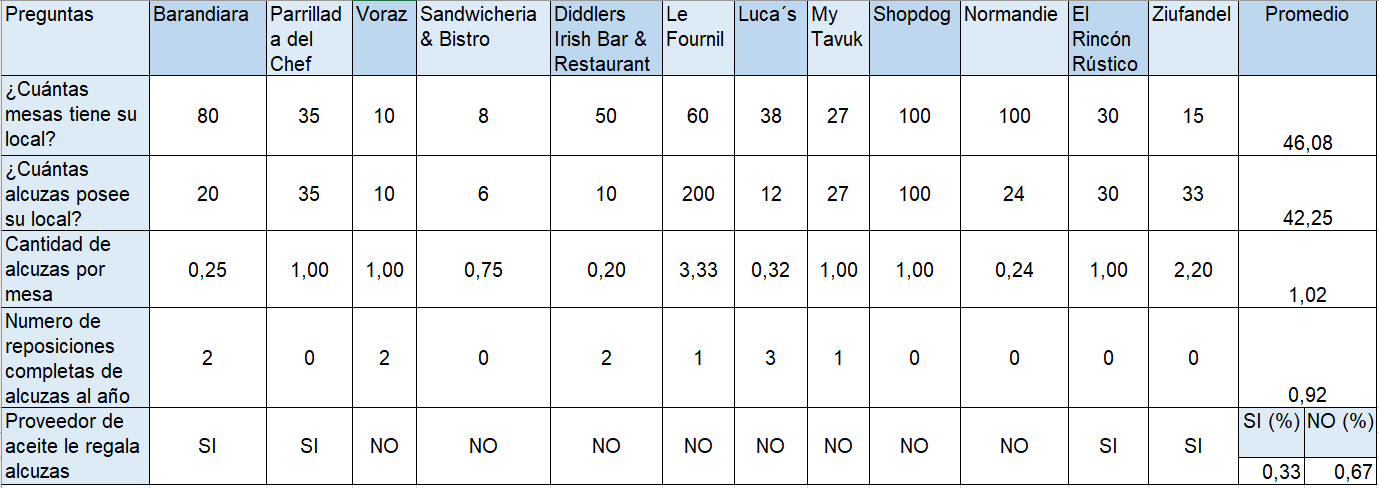
\includegraphics[width=\textwidth]{ResumenEntrevistasRestaurantes.png}
\caption{Resumen de resultados de entrevistas a restaurantes.}
\end{table}

\newpage
\subsection{Resultados de entrevistas a restaurantes.} \label{ResEntRest}
\begin{table}[H]
\centering
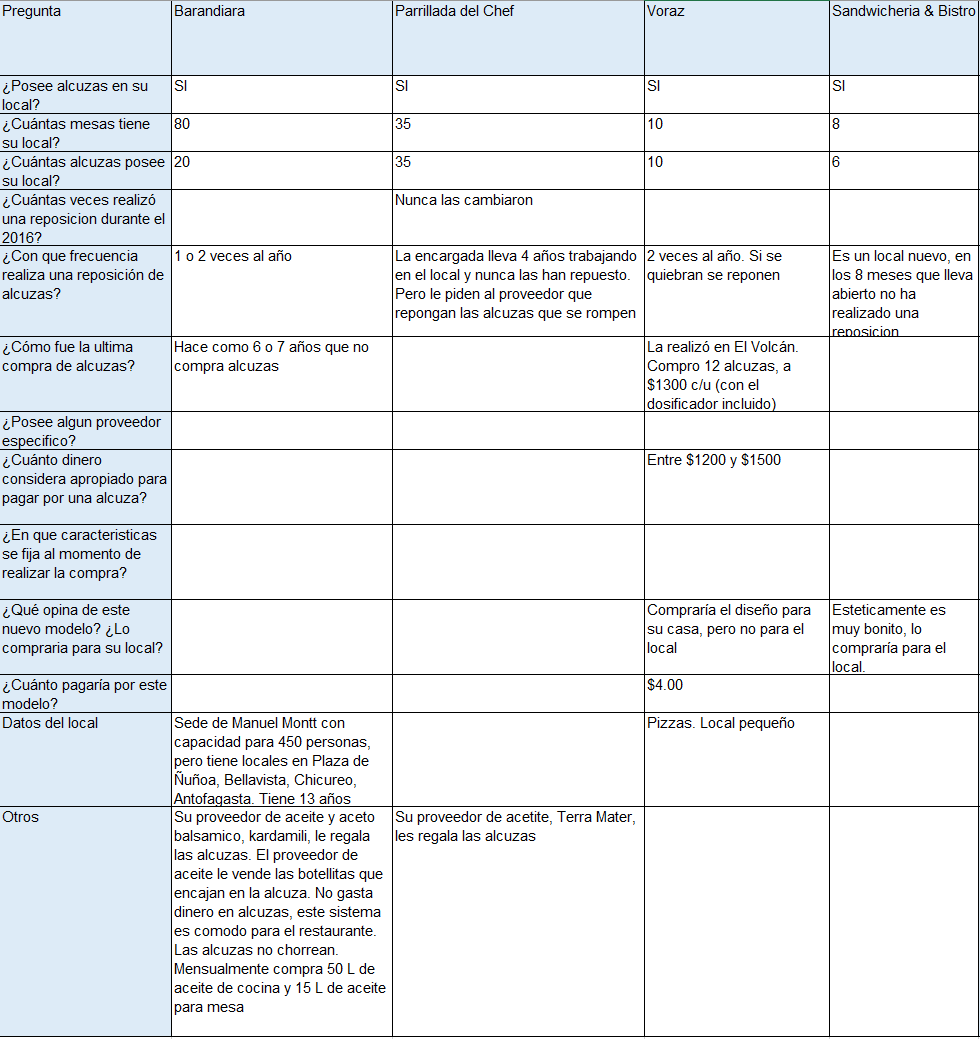
\includegraphics[width=\textwidth]{ResEntRestDetalle1.png}
\caption{Detalle de resultados de entrevistas a restaurantes (parte 1 de 3)}
\label{ResEntRestDetalle1}
\end{table}

\begin{table}[H]
\centering
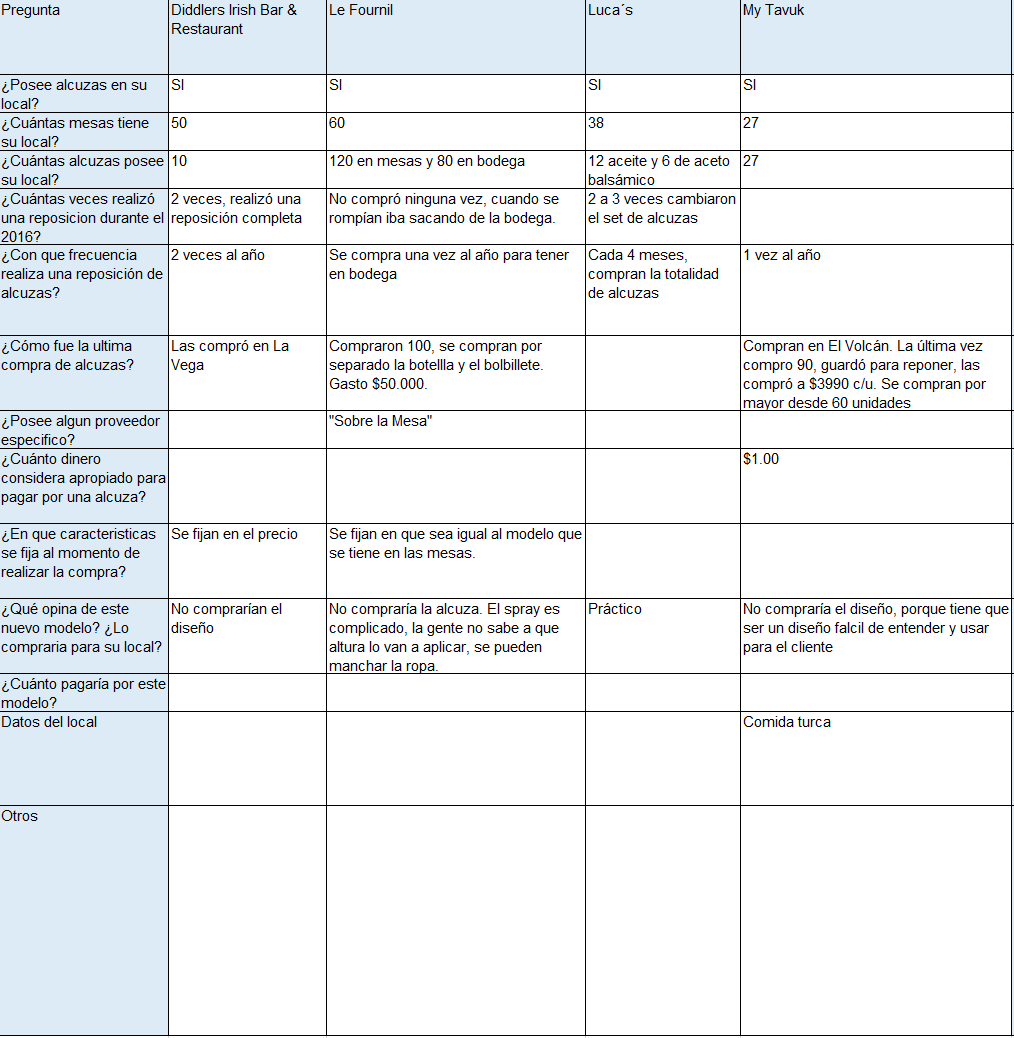
\includegraphics[width=\textwidth]{ResEntRestDetalle2.png}
\caption{Detalle de resultados de entrevistas a restaurantes (parte 2 de 3)}
\label{ResEntRestDetalle2}
\end{table}

\begin{table}[H]
\centering
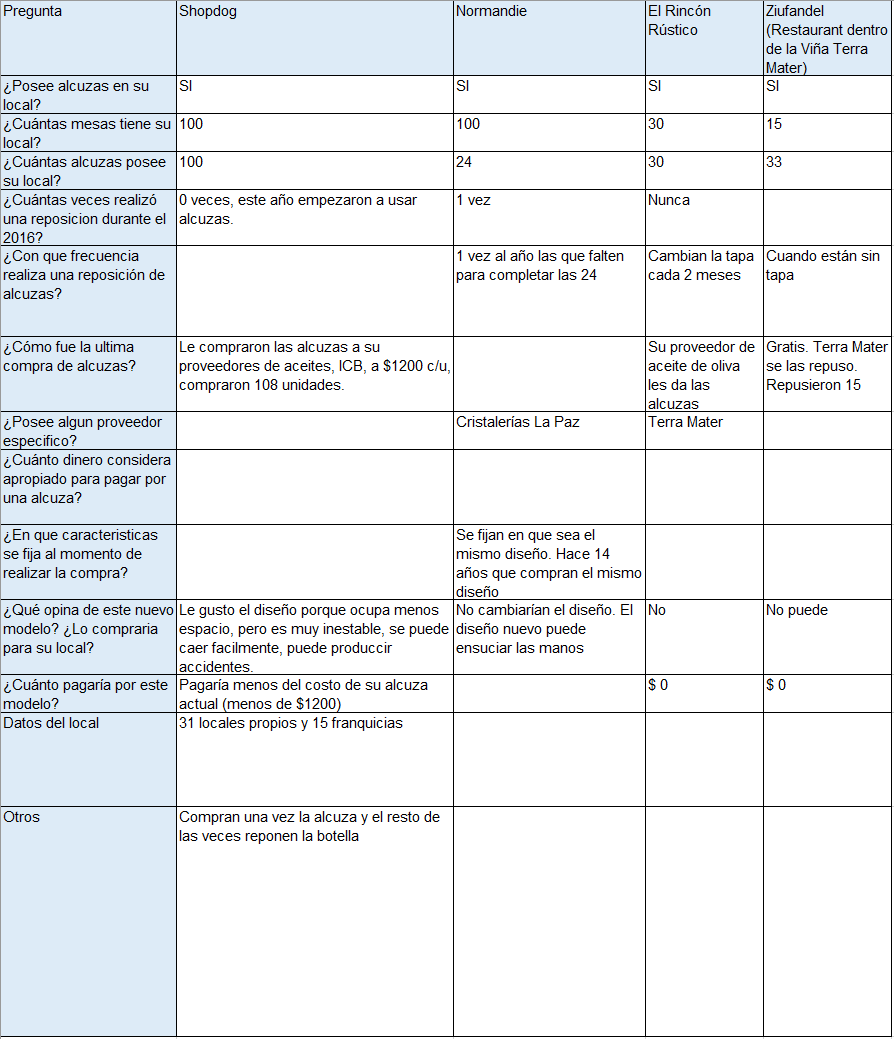
\includegraphics[width=\textwidth]{ResEntRestDetalle3.png}
\caption{Detalle de resultados de entrevistas a restaurantes (parte 3 de 3).}
\label{ResEntRestDetalle3}
\end{table}

\newpage
\subsection{Pauta de preguntas de la encuesta} \label{PauEnc}
\begin{enumerate}
\item ¿Qué edad tiene?

Respuesta abierta.

\item Género:
\begin{itemize}
\item[a)] Femenino.
\item[b)]      Masculino.
\end{itemize}
\item Estado civil:
\begin{itemize}
\item[a)] Casado/a o vive con su pareja.
\item[b)] Viudo/a.
\item[c)] Divorciado/a.
\item[d)] Separado/a.
\item[e)] Soltero/a, nunca se ha casado.
\item[f)] No contesta.
\end{itemize}
\item ¿Cuál es su ocupación?
\begin{itemize}
\item[a)]. Empleador.
\item[b)] Trabajador independiente o cuenta propia.
\item[c)] Trabajador/a de la administración pública.
\item[d)] Trabajador/a de empresa privada.
\item[e)] Servicio doméstico.
\item[f)] Trabajo no remunerado / responsable de las compras y el cuidado de la casa.
\item[g)] Estudiante.
\item[h)]Temporalmente no trabaja.
\item[i)] Retirado pensionado.
\item[j)] No sabe / No responde.
\end{itemize}
\item ¿Cuál es su nivel educacional?
\begin{itemize}
\item[a)] Sin estudios.
\item[b)] Básica incompleta.
\item[c)] Básica completa.
\item[d)] Media incompleta o Media técnica incompleta.
\item[e)] Media completa o Técnica incompleta.
\item[f)] Universitaria incompleta o Técnica completa.
\item[g)] Universitaria Completa.
\item[h)] Post Grado (Master, Doctorado o equivalente).
\item[i)] Sin respuesta.
\end{itemize}
\item ¿Sabe qué es una alcuza?
\begin{itemize}
\item[a)] Sí.
\item[b)]   No.
\end{itemize}
Explicar qué es una alcuza:
La alcuza es un sistema compuesto por dos frascos para aceite y vinagre generalmente (o aceto balsámico. (Adaptación de la RAE ).
\item ¿Tiene una alcuza en su casa?
\begin{itemize}
\item[a)] Sí.
\item[b)]     No.
\end{itemize}
\item ¿Utiliza a diario la alcuza en su casa al momento de comer?
\begin{itemize}
\item[a)] Sí.
\item[b)] No.
\end{itemize}
\item ¿Cuándo fue la última vez que compro una alcuza para su casa?
\begin{itemize}
\item[a)] Hace menos de 6 meses.
\item[b)] Hace 1 año.
\item[c)] Hace 2 años.
\item[d)] Hace 3 años.
\item[e)] Hace 5 años.
\item[f)] Hace 8 años.
\item[g)] Hace 10 años.
\item[h)] Nunca.
\end{itemize}
\item Durante el 2016, ¿Cuantas veces compró una alcuza?
\begin{itemize}
\item[a)]  0
\item[b)] 1
\item[c)] 2
\item[d)] 3
\item[e)] 4
\end{itemize}
\item ¿Cuánto dinero pagaría por una alcuza?
\begin{itemize}
\item[a)] \$0
\item[b)]     Más de \$0 hasta \$4.000
\item[c)]        Más de \$4.000 hasta \$8.000
\item[d)]        Más de \$8.000 hasta \$12.000
\item[e)]        Más de \$12.000 hasta \$16.000
\item[f)]         Más de \$16.000 hasta \$20.000
\item[g)]         Más de \$20.000
\end{itemize}
\item Al momento de comprar una alcuza ¿qué es lo primero que toma en consideración?
\begin{itemize}
\item[a)] Me basta con que sea una alcuza.
\item[b)]     Diseño estético y novedoso.
\item[c)]        Diseño práctico.
\item[d)]        Otro.
\end{itemize}
\item ¿En qué lugar compró o compraría una alcuza?
\begin{itemize}
\item[a)] Tiendas de casa comercial (Homecenter, Casa\&ideas, Easy, Falabella, Ripley).
\item[b)]      Comercio pequeño.
\item[c)]        Supermercados.
\item[d)]        Tienda especializada en artículos gourmet.
\item[e)]        Otro.
\end{itemize}
\item ¿Cuánto dinero pagaría por este diseño de alcuza? (mostrar diseño)
\begin{itemize}
\item[a)] \$0
\item[b)]     Más de \$0 hasta \$4.000
\item[c)]        Más de \$4.000 hasta \$8.000
\item[d)]        Más de \$8.000 hasta \$12.000
\item[e)]        Más de \$12.000 hasta \$16.000
\item[f)]         Más de \$16.000 hasta \$20.000
\item[g)]         Más de \$20.000
\end{itemize}
\end{enumerate}


\newpage
\subsection{Resultados de la encuesta a personas} \label{ResEncPer}

\begin{table}[H]
\centering
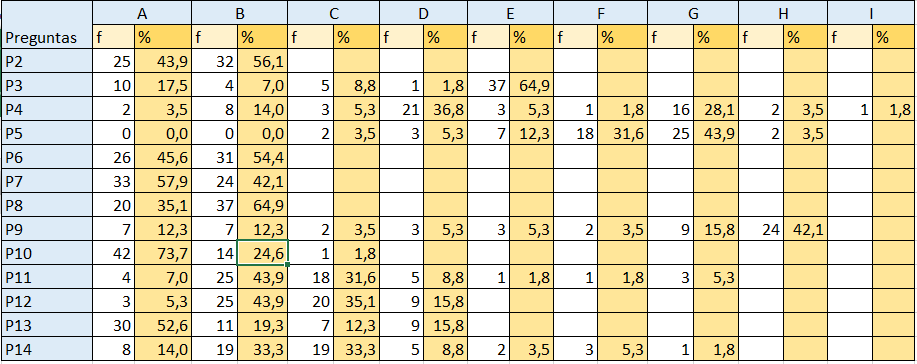
\includegraphics[width=\textwidth]{RespuestaEncPer.png}
\caption{Resultados de la encuesta a personas. Simbología: f = frecuencia, \% = porcentaje.}
\label{RespuestaEncPer}
\end{table}


\newpage
\subsection{Entrevistas empresas productoras de aceite - Pauta de preguntas}
\label{PauEntEmpAce}

\begin{enumerate}
\item ¿Cuál es su proveedor de envases de vidrio?
\item Aproximadamente, ¿cuántos envases de vidrio compra mensualmente?
\item  ¿Su empresa le regala o vende alcuzas a los restaurantes?
\item ¿Su empresa es proveedor de restaurantes? Si lo es, puede sugerir algunos nombres.
\item En el caso de que su empresa sí tenga un servicio que regala o vende alcuzas a restaurantes:
\begin{itemize}
\item ¿Con qué frecuencia regala o vende alcuzas?
\item ¿Su empresa se encarga de la fabricación de las alcuzas o las compra a un proveedor?
\item Si su empresa compra alcuzas, ¿cuál es su proveedor de alcuzas?. Aproximadamente, ¿cuántas alcuzas compra mensualmente?
\item Si su empresa confecciona las alcuzas, ¿cómo lo realizó? ¿A quién encomendó la fabricación de la matriz? ¿Qué empresa produce el envase de vidrio?
\end{itemize}
\item ¿Qué opina del diseño diseño de alcuza integrada? (Previamente se muestra una imagen y se explica su funcionamiento)
\end{enumerate}



\subsection{Respuestas de entrevistas a empresas de aceite.}
 \label{ResEntEmpAce}

Empresa: DELEYDA -Olivos Ruta del Sol S.A.

Entrevistado:Fernando Carrasco Spano (Commercial Director).

\begin{enumerate}
\item ¿Su empresa es proveedor de restaurantes? Si lo es, puede sugerir algunos nombres.

No lo somos.

\item ¿Cuál es su proveedor de envases de vidrios?

Cristalerías Toro.

 \item Aproximadamente ¿Cuántos envases de vidrio compra mensualmente?

45.000 Botellas

 \item ¿Su empresa le regala o vende alcuzas a los restaurantes?

No.

\item ¿Cree que sería un aporte positivo a su empresa agregar el servicio que venda alcuzas o las regale?

 Poder dar a conocer la marca, el aceite de oliva aún es muy comoditizado.

\item ¿Qué opina del diseño que se muestra en la imagen adjunta y el video?

 Precioso diseño.

\end{enumerate}

Empresa: Las200

Entrevistado: Feranda Fache (Brand Manager).

\begin{enumerate}
\item ¿Su empresa es proveedor de restaurantes? Si lo es, puede sugerir algunos nombres.

Son proveedores directos de restaurantes, tiene una lista confidencial.

\item ¿Cuál es su proveedor de envases de vidrios?

Proveedor de envases de vidrio: Cristalerías Toro.

\item ¿Su empresa le regala o vende alcuzas a los restaurantes?

Mandan a hacer su propia alcuza. Se mandó a hacer el diseño y la matriz se mandó a hacer en China y luego Cristalerías Toro hace las botellitas para la alcuza. La alcuza es de base de madera con dos botellas con el logo de la empresa. Solo le venden las alcuzas a cierto número de clientes, de forma exclusiva.

\item ¿Qué opina del diseño que se muestra en la imagen adjunta y el video?

Respecto del diseño de la alcuza que le mostré: no le gustó el diseño, no es práctico.
\end{enumerate}

\newpage
\subsection{Participación de mercado.}
 \label{PartMerc}
  \begin{figure}[H]
    \label{TablaPartMerc}
    \centering
    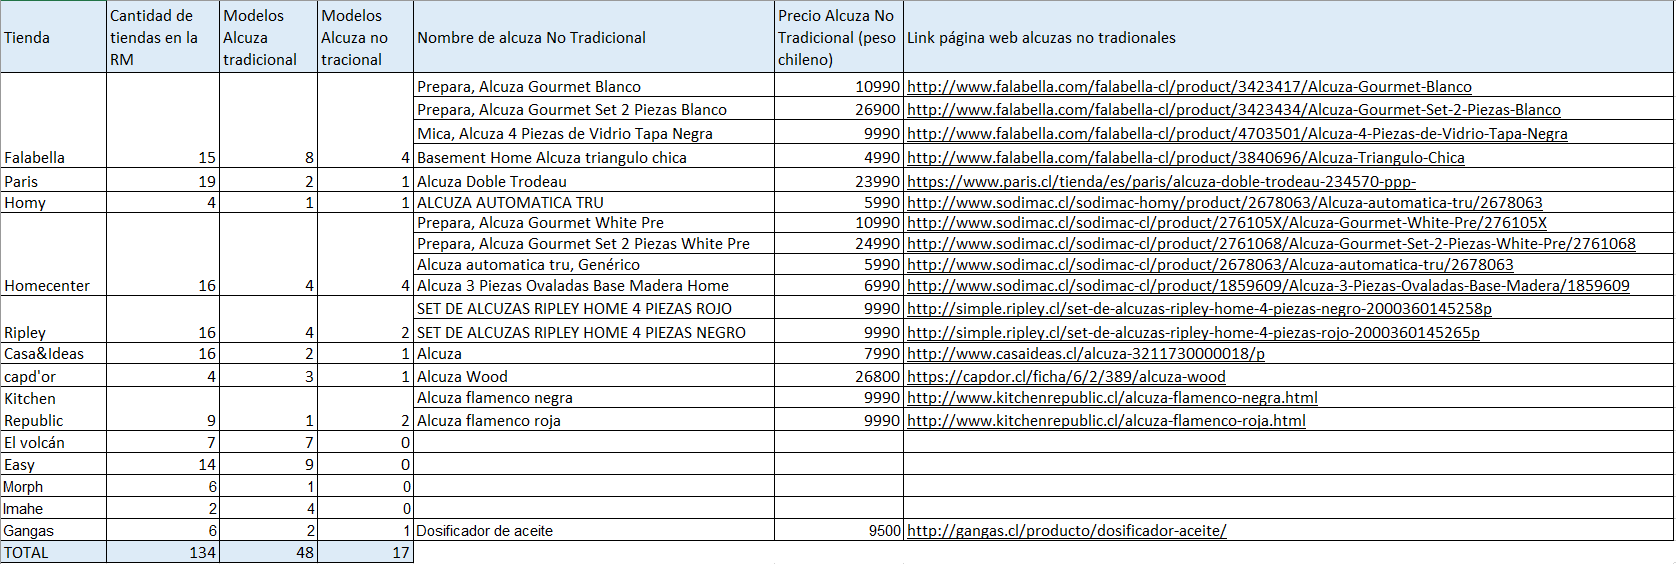
\includegraphics[width=1.3\textwidth , angle=90,origin=c]{TablaPartMerc.png}
    \caption{Participación de mercado.}
  \end{figure}
